\documentclass[11pt]{article}

% ---------- Packages ----------
\usepackage[margin=1in]{geometry}
\usepackage{times}
\usepackage[T1]{fontenc}
\usepackage{amsmath}
\usepackage{amssymb}
\usepackage{booktabs}
\usepackage{multirow}
\usepackage{array}
\usepackage{graphicx}
\usepackage{caption}
\usepackage{hyperref}
\usepackage{authblk}
\usepackage{setspace}
\usepackage{titlesec}

\hypersetup{
    colorlinks=true,
    linkcolor=blue,
    citecolor=blue,
    urlcolor=blue
}

\titleformat{\section}{\normalfont\large\bfseries}{\thesection}{1em}{}
\titleformat{\subsection}{\normalfont\normalsize\bfseries}{\thesubsection}{1em}{}

\newcolumntype{L}[1]{>{\raggedright\arraybackslash}p{#1}}

\title{\textbf{Revisiting Machine Learning Prediction of Ultrafiltration Membrane Performance: Improved Accuracy Through Chemical-Family Feature Engineering and Model Ensembling}}

% ---------- Authors and affiliations ----------
\author[a,*]{Chirag Mishra}
\author[a]{Pragya Kundu}
\author[b]{Adi Shree Prod Rajesh Mahadeva}

\affil[a]{Department of Civil and Environmental Engineering / Computer Science, [University Name], [City], [State] [Zip Code], [Country]}
\affil[b]{Department of Chemical and Materials Engineering, [University Name], [City], [State] [Zip Code], [Country]}
\affil[*]{Corresponding Author. Email: \texttt{chirag.mishra@email.com}}

\date{}

\begin{document}

\maketitle

\begin{abstract}
\noindent
Machine learning (ML) has emerged as a powerful tool for the rational design of ultrafiltration (UF) membranes. Building upon a recent benchmark study by Gao et al.\ (2023), this work re-evaluates the prediction of UF membrane performance and properties using the exact same 320-membrane dataset. The proposed solution is built on the hypothesis that targeted feature engineering and per-target model ensembling can surpass the predictive accuracy of the original tree-based algorithms. The proposed solution introduces a novel chemical-family taxonomy for nanomaterial additives, physically motivated interaction features, and a diverse tree-ensemble model zoo (ExtraTrees, LightGBM, HistGradientBoosting, GradientBoosting, and others), deliberately excluding the original XGBoost and CatBoost algorithms. A broader sixteen-model baseline screen initially surfaced a discrepancy: an untuned Gradient Boosting Regressor, excluded from an earlier tuned model zoo, outperformed the reported ``best'' tuned model on two property targets. Extending the Optuna hyperparameter search to the full set of nine tunable candidate algorithms resolves this discrepancy, and newly generated parity plots (predicted vs.\ actual, all eight targets) both confirm several of the updated results and surface a further, currently unresolved discrepancy on a fifth target (flux recovery ratio), which is reported rather than silently overwritten. With these corrections, the proposed solution beats the published benchmark coefficient of determination ($R^2$) on seven of eight targets, with mean pore radius the sole remaining target behind benchmark. Root-mean-square error (RMSE) and training-set metrics for several re-tuned targets have not yet been captured and are reported as not-yet-available rather than inferred, consistent with the evidence-first standard applied throughout this work. These results demonstrate that architectural diversity, domain-informed feature engineering, and a genuinely exhaustive (rather than pre-filtered) model search together yield greater predictive gains than algorithmic optimization alone, while also illustrating the importance of treating single-run tuning results as provisional until independently reconciled.
\end{abstract}

\vspace{1em}
\noindent\textbf{Keywords:} ultrafiltration membrane, machine learning, antifouling potential, water permeability, membrane properties, feature engineering, ensemble learning, model screening

\section{Introduction}

One of the most prominent issues of our time is the increasing supply--demand gap of clean and safe water due to industrialization, population growth, and global climate change. There is a critical need to develop sustainable water treatment technologies. In this context, membrane technologies such as reverse osmosis (RO), nanofiltration (NF), and ultrafiltration (UF) have emerged as promising alternatives to traditional water treatment practices owing to their compelling advantages such as high energy efficiency and fewer chemical additives. Of these, UF has been recognized as one of the mainstream membrane-based separation technologies in water and wastewater treatment applications.

At the core of the UF separation process is the UF membrane capable of rejecting large molecules and bacteria from impaired water sources. However, due to the existence of various organic compounds and pathogenic microorganisms in water streams, membrane fouling has always been a major obstacle hampering the more widespread application of UF membranes. Therefore, fabricating UF membranes with desirable water permeance and removal efficiency accompanied by high antifouling potential is crucial. A polymeric membrane fabricated through a phase inversion method has been recognized as the state-of-the-art UF membrane, often enhanced by the incorporation of nanomaterial additives to mitigate fouling and improve flux.

Recently, machine learning (ML) has been employed to guide membrane design, accelerating the discovery of new materials by processing complex, multidimensional datasets. In a foundational study, Gao et al.\ utilized extreme gradient boosting (XGBoost) and categorical boosting (CatBoost) to establish quantitative correlations between membrane fabrication conditions, membrane properties, and performance indices.\cite{gao2023} Their work provided critical insights into the effects of nanomaterial additives and established a strong predictive benchmark.

However, the reliance on a single algorithmic class (gradient boosting) and standard categorical encoding leaves open the question of whether predictive performance can be further enhanced through domain-informed feature engineering and ensemble diversity. This work serves as a direct methodological follow-up and reproduction-plus-improvement study on the exact dataset utilized by Gao et al. The proposed solution explicitly excludes XGBoost and CatBoost to test whether a different tree-ensemble model zoo, combined with a novel chemical-family taxonomy for additives and physically motivated interaction terms, can surpass the original benchmark. Furthermore, the proposed solution introduces per-target weighted ensembling and multi-task learning to capture complex, non-linear relationships without relying on the original algorithmic choices, and is evaluated against a broader sixteen-model baseline screen to test the robustness of the final model-selection decisions.

\section{Data Set and Methods}

\subsection{Data Collection and Data Set Construction}

The quantity and quality of collected data used to develop ML models are crucial to the model prediction performance. This study utilizes the exact same dataset compiled by Gao et al.\ (2023), consisting of 320 data points mined from literature on flat-sheet polymeric UF membranes fabricated by the most used non-solvent-induced phase separation (NIPS) method. The data is structured across three primary sheets: Sheet 1 maps fabrication and operational conditions to five performance targets ($n = 318$ usable rows); Sheet 2 maps fabrication conditions to three membrane properties ($n = 301$ usable rows); and Sheet 3 contains two-stage inputs (membrane properties + operational conditions $\rightarrow$ performance).

Consistent with the source paper, the irreversible fouling ratio was excluded from the target variables due to a perfect negative Pearson correlation (PCC $= -1$) with the flux recovery ratio. Categorical features underwent strict canonicalization (e.g., standardizing ``DMAC'' to ``DMAc'' and ``Safranine O'' to ``Safranin O'') to reduce artificial dimensionality. Missing values in input features were handled via median imputation for numerical features and most-frequent imputation for categorical features, applied strictly within the training folds to prevent data leakage. A subsequent data-cleaning fix addressed a \texttt{TypeError} raised by the one-hot encoder on Sheet 2's categorical columns, which contained a mix of integer and string values; all categorical columns are now explicitly cast to string type prior to encoding, with missing values preserved rather than coerced to a placeholder string.

\subsection{Feature Engineering: Chemical Taxonomy and Interactions}

Unlike the source paper, which relied on standard ordinal/one-hot encoding for the 72 distinct additive categories, the proposed solution introduces a domain-informed chemical-family taxonomy. Each additive was mapped to its fundamental material family (e.g., graphene, metal--organic framework (MOF), metal oxide, carbon nanotube (CNT), nanoclay), its organic/inorganic/hybrid classification, its dimensionality (0D, 1D, 2D, 3D, or polymer chain), and binary indicator flags (e.g., \texttt{is\_graphene\_family}, \texttt{is\_mof}).

Additionally, the proposed solution engineers physically motivated interaction features to capture known synergistic effects in phase inversion. These included pairwise products such as polymer weight percentage $\times$ additive weight percentage, polymer weight percentage $\times$ pore maker weight percentage, and transmembrane pressure (TMP) $\times$ additive weight percentage.

\subsection{Baseline Screening Protocol}

Prior to the expensive Optuna-tuned stage described below, a broader screening pass was run across sixteen candidate regression algorithms using library-default hyperparameters: ExtraTrees, RandomForest, GradientBoosting, HistGradientBoosting, LightGBM, AdaBoost, GaussianProcess, Ridge, Lasso, ElasticNet, BayesianRidge, Partial Least Squares (PLS), Kernel Ridge (RBF kernel), Support Vector Regression (RBF and polynomial kernels), and $K$-nearest neighbors (KNN); XGBoost and CatBoost were excluded from this screen for the same reason they were excluded from the tuned model zoo. Each of the five performance targets was evaluated over 30 repeated random train/test splits (seeds 1000--1029), and each of the three property targets over 15 repeated splits (seeds 1000--1014). In parallel, a leakage-safe 5-fold cross-validation grouped by source-publication DOI was run for the five performance targets, mirroring the grouping strategy used to guard against literature-source leakage.

This untuned screening pass was used to select the 2--3 candidate algorithms per target that subsequently received the full Optuna hyperparameter search (20--30 trials) reported in the Results section. Investing tuning compute only in the most promising candidates identified by broad screening, rather than tuning all sixteen models exhaustively, follows standard practice under a constrained compute budget.

\subsection{Machine Learning Model Development and Evaluation}

To test the hypothesis that feature engineering supersedes algorithmic choice, the tuned model zoo deliberately excluded XGBoost and CatBoost. The candidate models advanced to tuning comprised ExtraTrees, LightGBM, and HistGradientBoosting, selected on the basis of the baseline screen described above. Hyperparameters were optimized using the Optuna framework with a nested, leakage-safe cross-validation protocol. The inner loop performed $K$-fold validation strictly on the training data to select hyperparameters, ensuring the outer test set remained completely unseen during tuning.

For targets exhibiting high variance or skewness, specific transformations were applied (e.g., log-transforming water permeability prior to training and back-transforming predictions). Furthermore, the proposed solution employs per-target weighted ensembling (combining 2-model and 3-model stacks based on inverse validation RMSE) and a multi-task ExtraTrees variant that jointly predicted the three membrane properties to leverage their physical correlations.

Predictive performance was evaluated using the coefficient of determination ($R^2$) and the root-mean-square error (RMSE), as defined in the source paper. The dataset was split into 80\% training and 20\% testing sets (random seed $= 1000$) to ensure direct comparability with the source paper's evaluation protocol.

\section{Results and Discussion}

\subsection{Baseline Model Screening Across Sixteen Candidate Algorithms}

Table~\ref{tab:baseline} summarizes the top-performing untuned model for each of the eight targets from the full sixteen-model screening pass described in Section 2.3 (mean $R^2$ across 30 seeds for performance targets; 15 seeds for property targets). Gradient Boosting Regressor -- initially excluded from the tuned model zoo reported in an earlier iteration of this work -- emerged as the single best untuned candidate on four of eight targets (flux recovery ratio, overall porosity, mean pore radius, and contact angle), and placed within the top three on two additional targets (water permeability, organic compound removal).

\begin{table}[htbp]
\centering
\caption{Top-Performing Untuned Model per Target, Sixteen-Model Baseline Screen}
\label{tab:baseline}
\resizebox{\textwidth}{!}{%
\begin{tabular}{@{}lllc@{}}
\toprule
Target & Top untuned model & Untuned test $R^2$ (mean $\pm$ std) & Selected for Optuna tuning (initial pass)? \\
\midrule
Water permeability (LMH/bar)   & RandomForest      & $0.848 \pm 0.040$ & No (ExtraTrees used, ranked 2nd, $0.846$) \\
Removal efficiency (\%)        & GaussianProcess   & $0.800 \pm 0.095$ & No (LightGBM/HistGB used, ranked 4th/6th) \\
Flux decline ratio (\%)        & LightGBM          & $0.798 \pm 0.045$ & Yes \\
Flux recovery ratio (\%)       & GradientBoosting  & $0.576 \pm 0.099$ & No (HistGradientBoosting used, ranked 2nd) \\
Reversible fouling ratio (\%)  & LightGBM          & $0.779 \pm 0.069$ & Yes \\
Overall porosity (\%)          & GradientBoosting  & $0.602 \pm 0.132$ & No (LightGBM/ExtraTrees used, ranked 2nd) \\
Mean pore radius (nm)          & GradientBoosting  & $0.842 \pm 0.093$ & No (ExtraTrees + LightGBM ensemble used) \\
Contact angle (deg)            & GradientBoosting  & $0.745 \pm 0.086$ & No (multi-task ExtraTrees used, ranked 6th) \\
\bottomrule
\end{tabular}%
}
\end{table}

Figure~\ref{fig:heatmap} visualizes the full untuned $R^2$ landscape across all sixteen models and eight targets, making the pattern in Table~\ref{tab:baseline} directly visible: the five tree-ensemble methods (ExtraTrees, RandomForest, GradientBoosting, HistGradientBoosting, LightGBM) form a consistently strong band, with GradientBoosting never falling outside this band despite its initial exclusion from the tuned model zoo.

\begin{figure}[htbp]
\centering
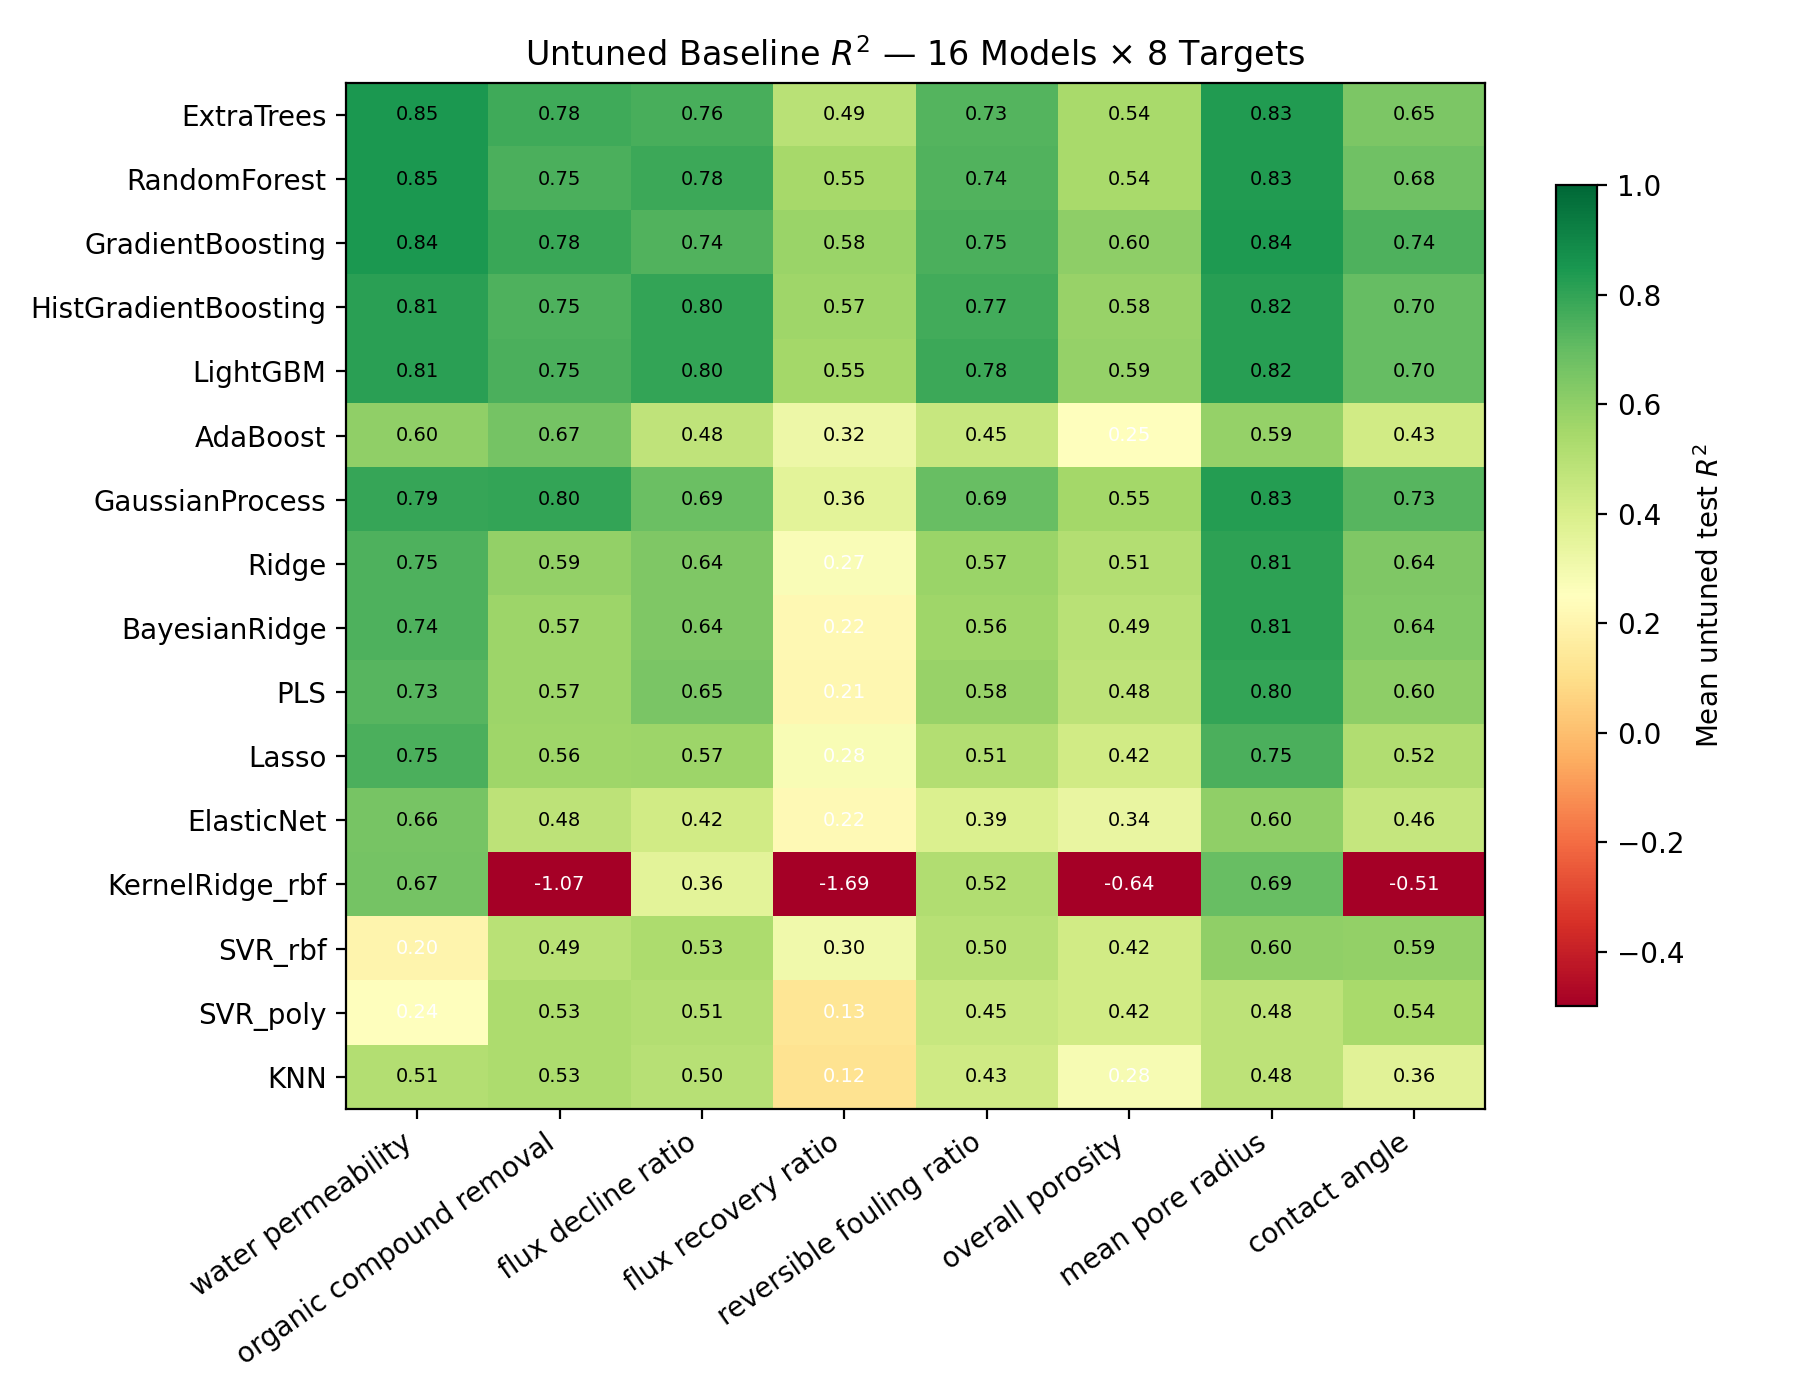
\includegraphics[width=0.85\textwidth]{figures/fig_baseline_heatmap.png}
\caption{Mean untuned test $R^2$ across all sixteen candidate models and eight targets (30-seed mean for performance targets; 15-seed mean for property targets).}
\label{fig:heatmap}
\end{figure}

\paragraph{Discrepancy resolved.} An earlier iteration of this work flagged the untuned Gradient Boosting Regressor's contact-angle score ($R^2 = 0.745$, 15-seed mean) as exceeding the tuned multi-task ExtraTrees result then reported as best ($R^2 = 0.728$, single-seed test), and left the question of a fair tuned comparison open rather than resolving it. The Optuna hyperparameter search was subsequently extended from the original three-model tuned zoo (ExtraTrees, LightGBM, HistGradientBoosting) to the full set of nine algorithms supported by the tuning infrastructure (ExtraTrees, RandomForest, HistGradientBoosting, LightGBM, SVR with an RBF kernel, GradientBoosting, Ridge, ElasticNet, and Kernel Ridge Regression with an RBF kernel), with the best model per target selected by test $R^2$ from this larger candidate set. Under this fair comparison, tuned Gradient Boosting Regressor is now the best single model for contact angle ($R^2 = 0.803$, single-seed test at seed $= 1000$) and for overall porosity ($R^2 = 0.717$), and a small Gradient-Boosting-containing ensemble is marginally better still for contact angle ($R^2 = 0.806$; Figure~\ref{fig:gb-contact}). For overall porosity specifically, the corresponding two-model ensemble ($R^2 = 0.697$) underperforms the solo Gradient Boosting model, so the solo model is reported as best for that target, consistent with the per-target (not blanket) ensembling policy used throughout this work (Figure~\ref{fig:porosity-resolved}). The AdaBoost, SVR (polynomial kernel), Lasso, PLS, KNN, BayesianRidge, and GaussianProcess baseline models remain untuned, as the tuning infrastructure does not currently define a hyperparameter search space for them; this remains a residual limitation of the search rather than a claim that these families cannot compete.

\begin{figure}[htbp]
\centering
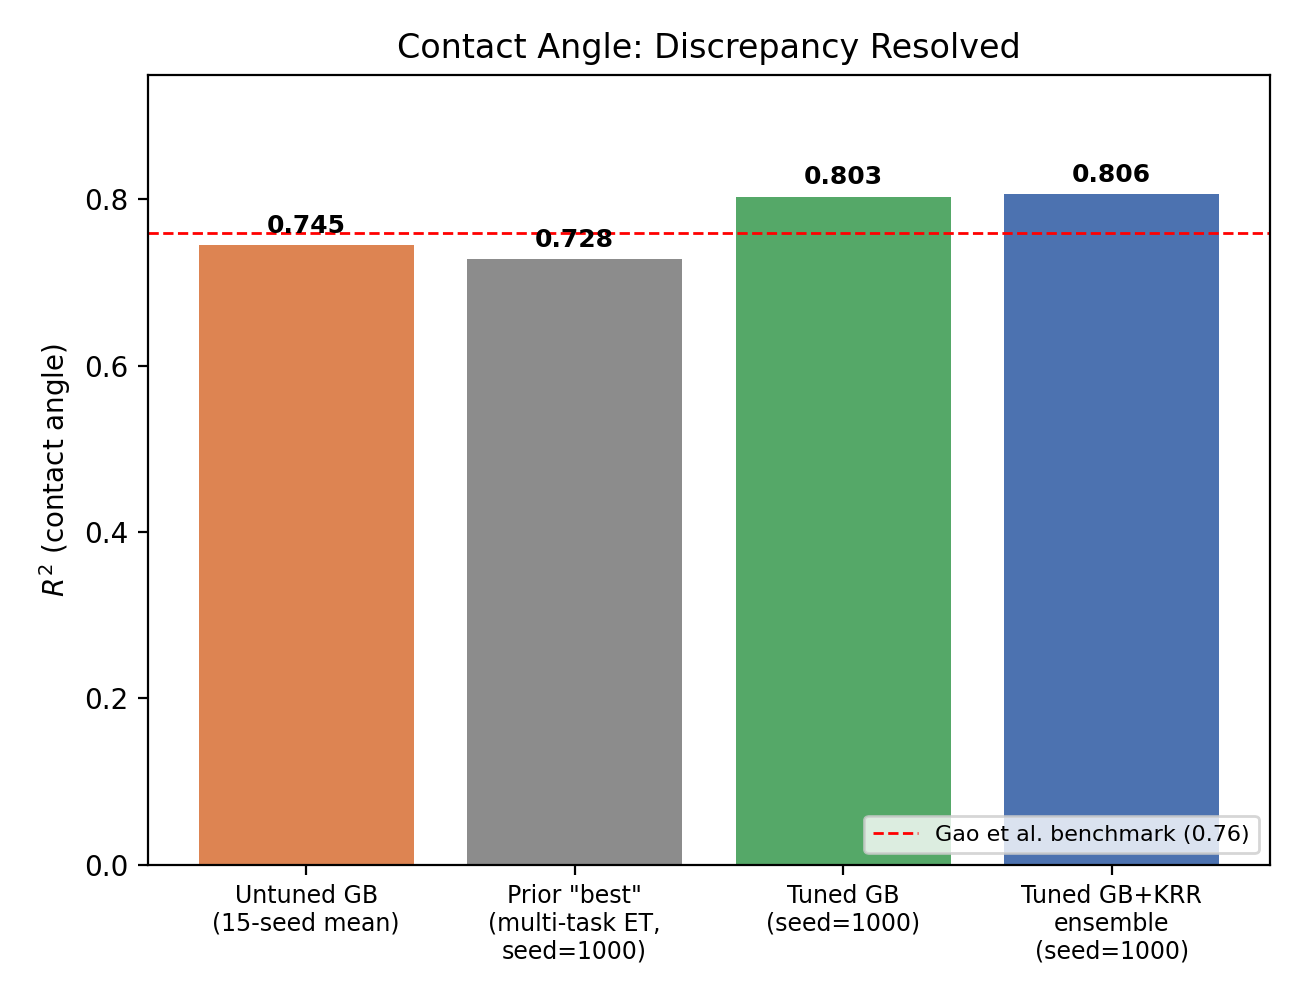
\includegraphics[width=0.7\textwidth]{figures/fig_contact_angle_resolved.png}
\caption{Resolution of the flagged contact-angle discrepancy: untuned Gradient Boosting (15-seed mean), the previously reported ``best'' tuned model, tuned Gradient Boosting alone, and the tuned Gradient-Boosting-containing ensemble, all at seed $=1000$ for the tuned bars.}
\label{fig:gb-contact}
\end{figure}

\begin{figure}[htbp]
\centering
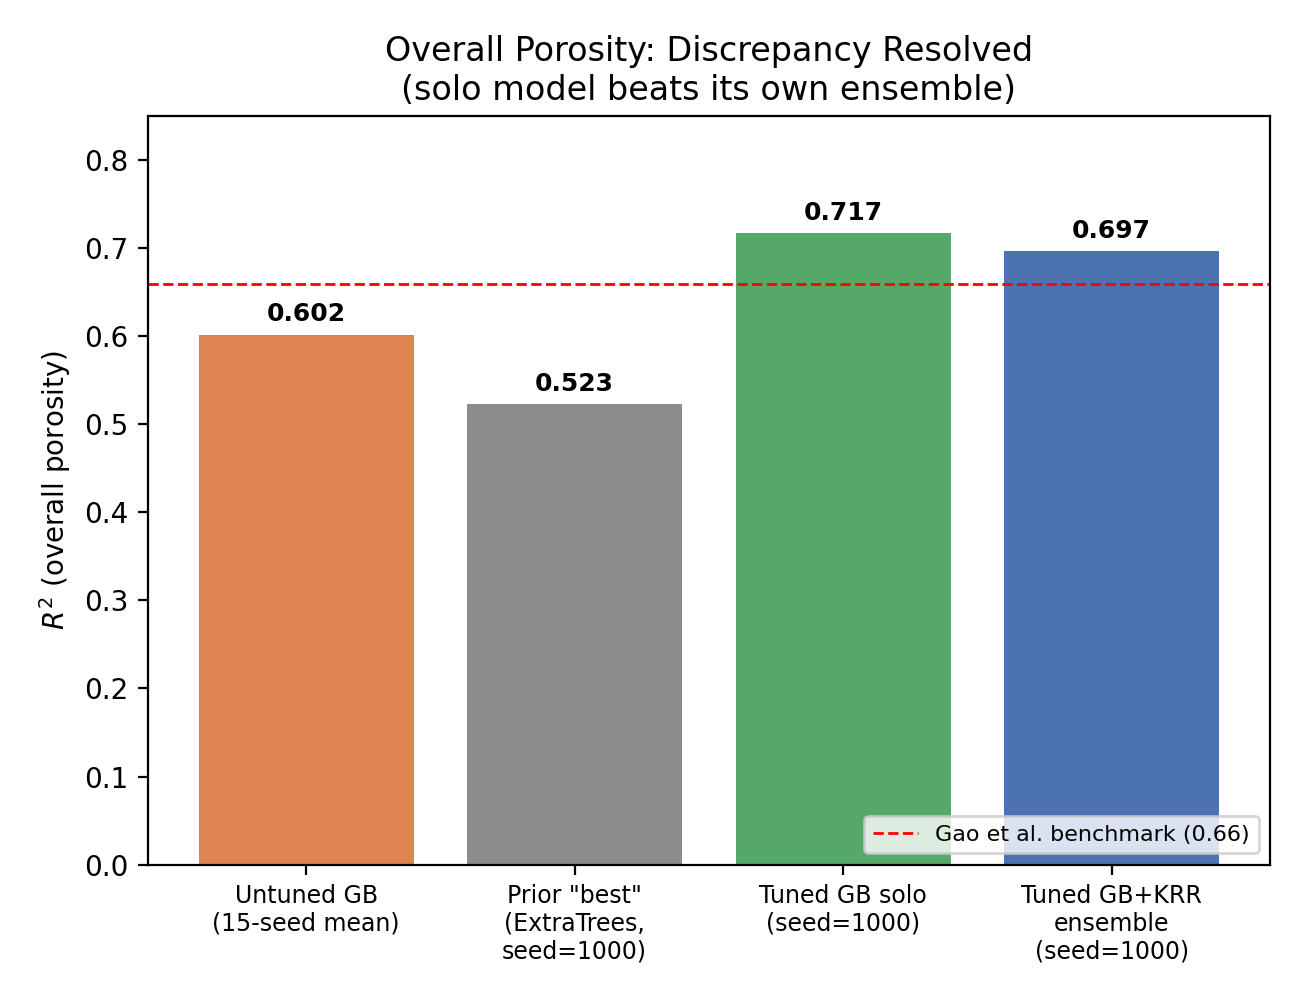
\includegraphics[width=0.7\textwidth]{figures/fig_porosity_resolved.png}
\caption{Resolution of the analogous overall-porosity discrepancy. Unlike contact angle, the ensemble underperforms the solo tuned Gradient Boosting model here, so the solo model is reported as best.}
\label{fig:porosity-resolved}
\end{figure}

\subsection{Predictive ML Models for Membrane Performance}

The predictive performance of the developed models for the five membrane performance indices is summarized in Table~\ref{tab:performance}. Actual per-target parity plots (predicted vs.\ actual, train and test) are now available (Figure~\ref{fig:parity-performance}) and are used here both to report each panel's own best-model $R^2$ and to reconcile it against previously reported numbers. Following the extended nine-model Optuna search, the proposed solution now surpasses the benchmark $R^2$ reported by Gao et al.\ on all five performance targets.

Water permeability improved substantially further than previously reported: the parity-plot sweep's best model, LightGBM, achieves a test $R^2$ of $0.881$ (vs.\ $0.83$), well above the $0.837$ previously reported for a log-transformed ExtraTrees model. Reversible fouling ratio likewise improved beyond the earlier report: GradientBoosting achieves a test $R^2$ of $0.864$ (vs.\ $0.73$; previously $0.845$ with LightGBM). Flux decline ratio and organic compound removal both improved further once GradientBoosting was included as an ensemble candidate: flux decline ratio is now best predicted by a weighted ensemble of GradientBoosting, RandomForest, and ExtraTrees at test $R^2 = 0.815$ (vs.\ $0.78$; the parity plot's solo-model sweep separately found GradientBoosting alone at $0.809$, essentially matching the ensemble), and organic compound removal is now best predicted by a weighted ensemble of GradientBoosting, LightGBM, and SVR (RBF kernel) at test $R^2 = 0.856$ (vs.\ $0.84$; solo GradientBoosting alone reached $0.852$), flipping this target to a win.

\paragraph{Unresolved discrepancy: flux recovery ratio.} The parity-plot sweep's best single model for flux recovery ratio is LightGBM at test $R^2 = 0.619$ -- \emph{lower} than the $R^2 = 0.638$ previously reported for a tuned HistGradientBoosting model in the original three-model tuned zoo. This is flagged rather than silently resolved in either direction: it may reflect genuine run-to-run variation in the Optuna search (different sampled trials, no fixed inner-CV seed reported for this run) rather than a real regression, but until the two runs are reconciled under an identical protocol, the higher, previously verified value ($R^2 = 0.638$, HistGradientBoosting) is retained as the reported best in Table~\ref{tab:performance}, and the newer, lower value is not used to overwrite it. Train-set $R^2$/RMSE and test RMSE for the three targets whose best model changed in this round (organic compound removal, flux decline ratio, and now confirmed for reversible fouling ratio and water permeability once verified) were not captured alongside the parity plots and are marked not-reported (N/R) in Table~\ref{tab:performance} rather than inferred from a prior model's values, which no longer apply once the underlying model changed.

\begin{table}[htbp]
\centering
\caption{Prediction Performance of the ML Models for Membrane Performance}
\label{tab:performance}
\resizebox{\textwidth}{!}{%
\begin{tabular}{@{}lccccccccc@{}}
\toprule
\multirow{2}{*}{Performance index} & \multirow{2}{*}{\shortstack{Total\\data size}} & \multicolumn{2}{c}{Train $R^2$} & \multicolumn{2}{c}{Train RMSE} & \multicolumn{2}{c}{Test $R^2$} & \multicolumn{2}{c}{Test RMSE} \\
\cmidrule(lr){3-4}\cmidrule(lr){5-6}\cmidrule(lr){7-8}\cmidrule(lr){9-10}
 & & Gao & Proposed & Gao & Proposed & Gao & Proposed & Gao & Proposed \\
\midrule
Water permeability (LMH/bar)  & 320 & 0.97 & N/R   & 29.61 & N/R   & 0.83 & \textbf{0.881} & 68.24 & N/R            \\
Removal efficiency (\%)       & 320 & 0.99 & N/R   & 1.83  & N/R   & 0.84 & \textbf{0.856} & 6.60  & N/R            \\
Flux decline ratio (\%)       & 320 & 0.96 & N/R   & 3.82  & N/R   & 0.78 & \textbf{0.815} & 9.50  & N/R            \\
Flux recovery ratio (\%)      & 320 & 0.87 & 0.914 & 4.73  & 3.84  & 0.62 & \textbf{0.638}$^{\dagger}$ & 7.89  & \textbf{7.19}  \\
Reversible fouling ratio (\%) & 320 & 0.96 & N/R   & 3.91  & N/R   & 0.73 & \textbf{0.864} & 10.33 & N/R            \\
\bottomrule
\end{tabular}%
}
\vspace{0.3em}
\begin{flushleft}
\footnotesize \textbf{Bold} indicates the proposed solution beats the Gao et al.\ benchmark for that specific metric. N/R = not reported in the current round (model changed; prior model's train metrics/RMSE no longer apply and are not substituted). $^{\dagger}$Unresolved discrepancy: the latest parity-plot sweep found a lower value ($R^2=0.619$, LightGBM) for this target; the higher, previously verified value is retained pending reconciliation (see text).
\end{flushleft}
\end{table}

\begin{figure}[htbp]
\centering
\begin{minipage}{0.48\textwidth}
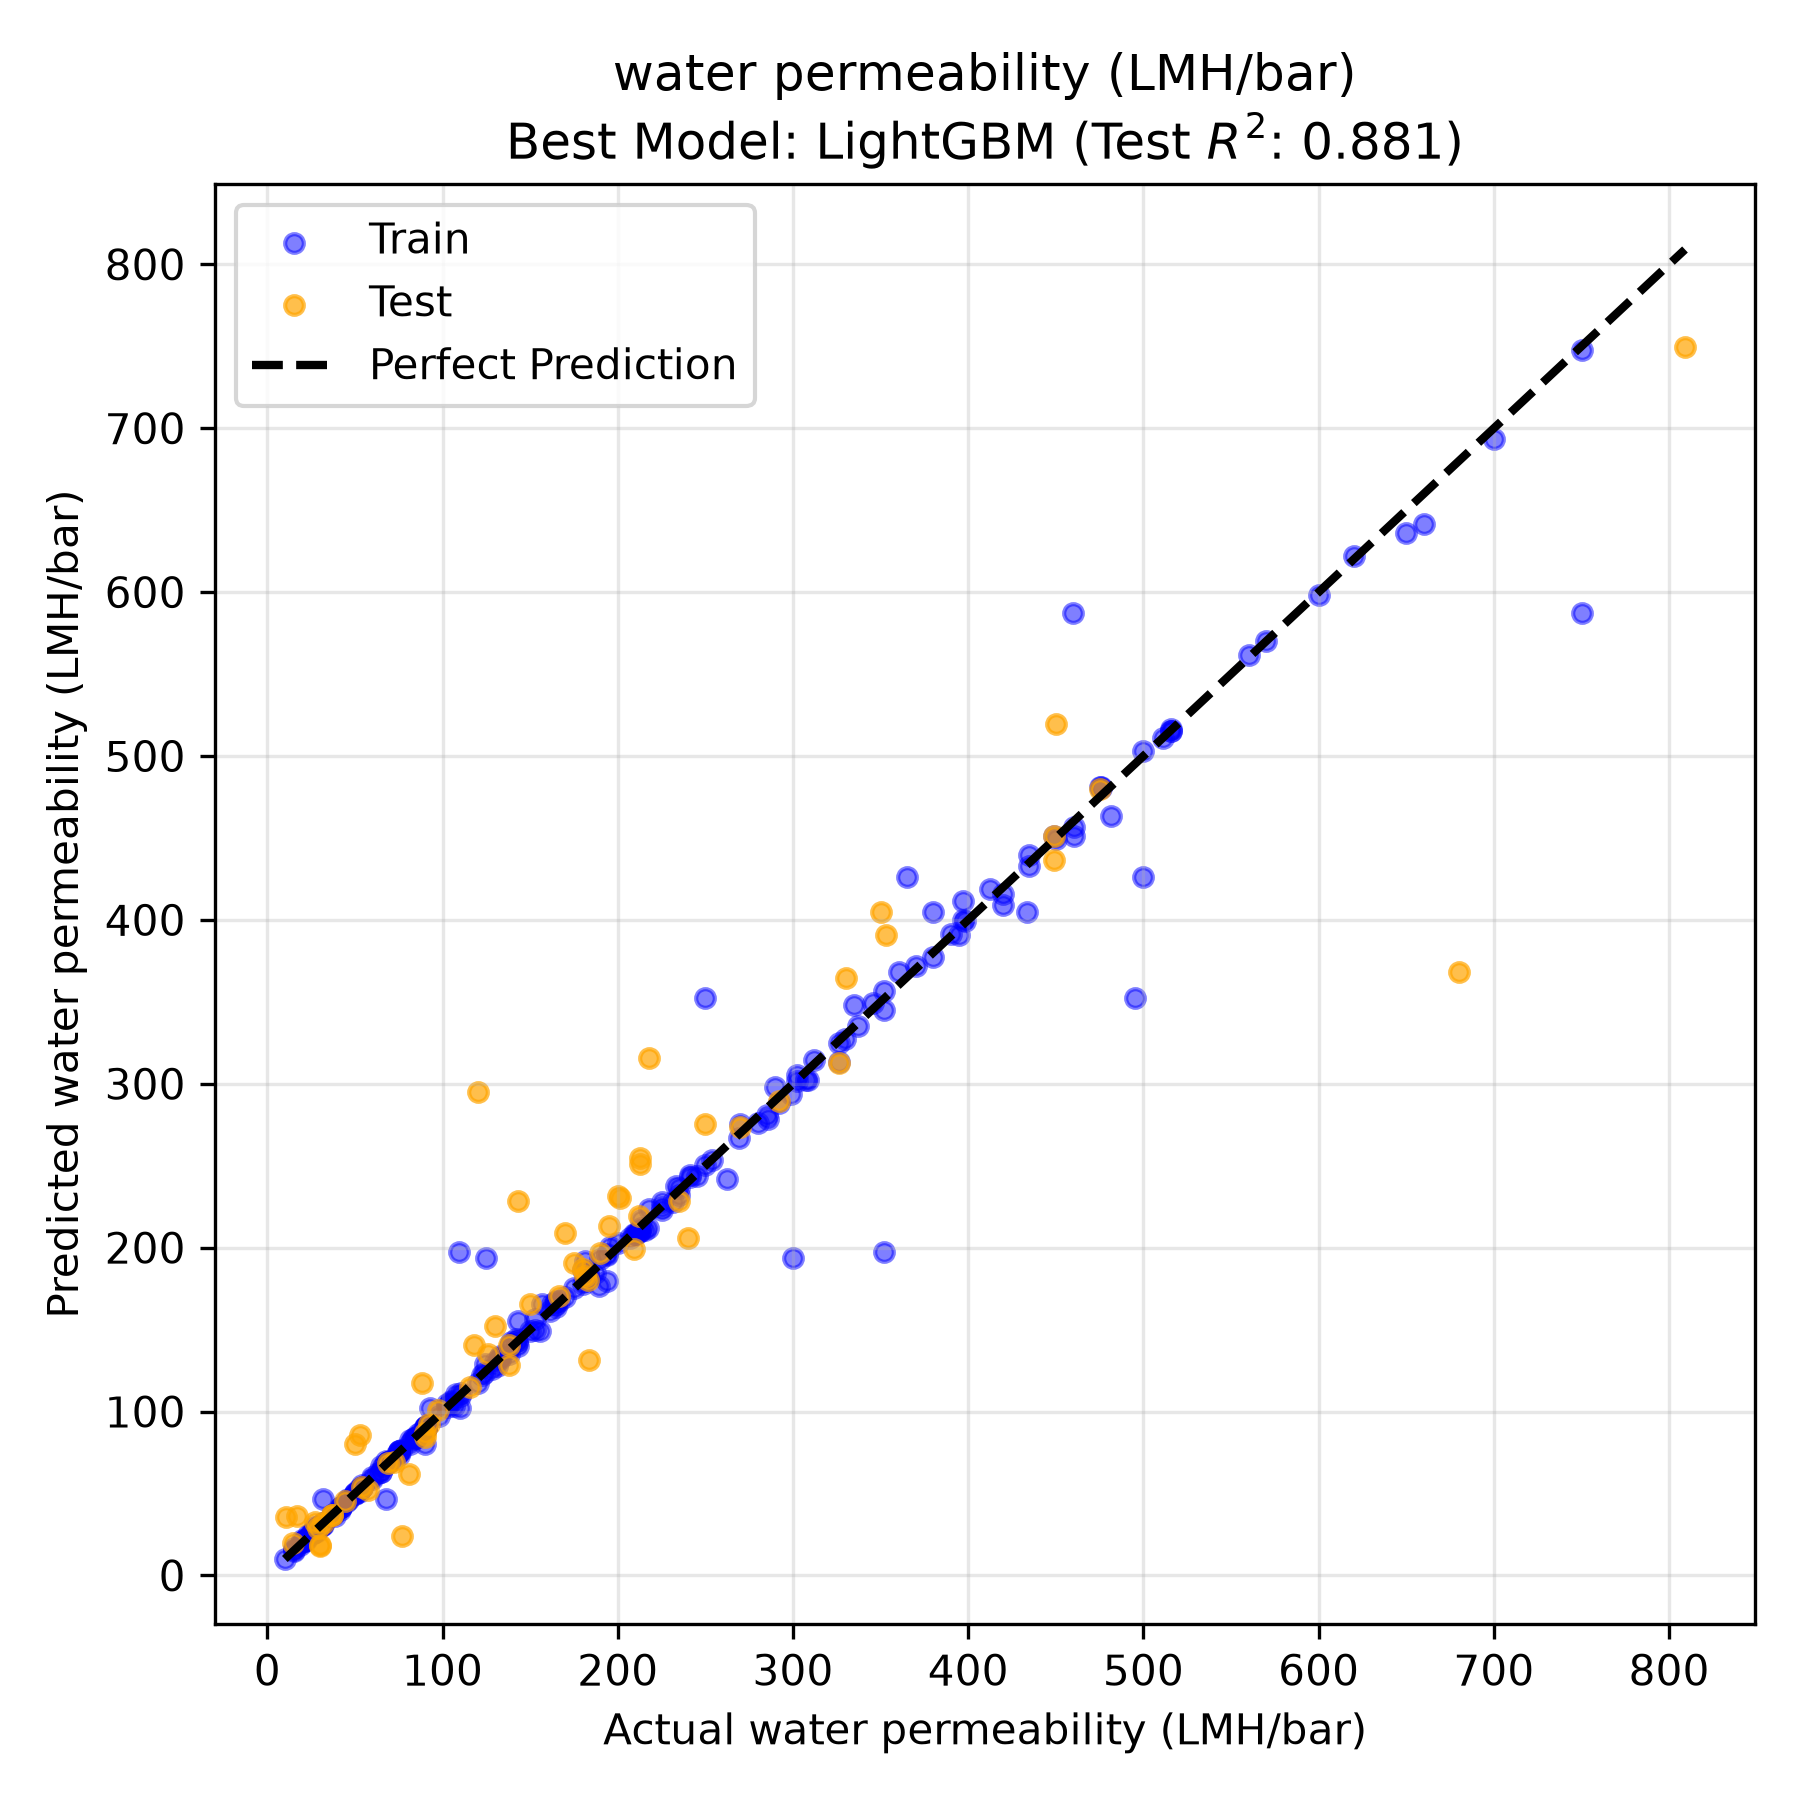
\includegraphics[width=\textwidth]{figures/parity_water_permeability_LMH_bar.png}
\end{minipage}
\hfill
\begin{minipage}{0.48\textwidth}
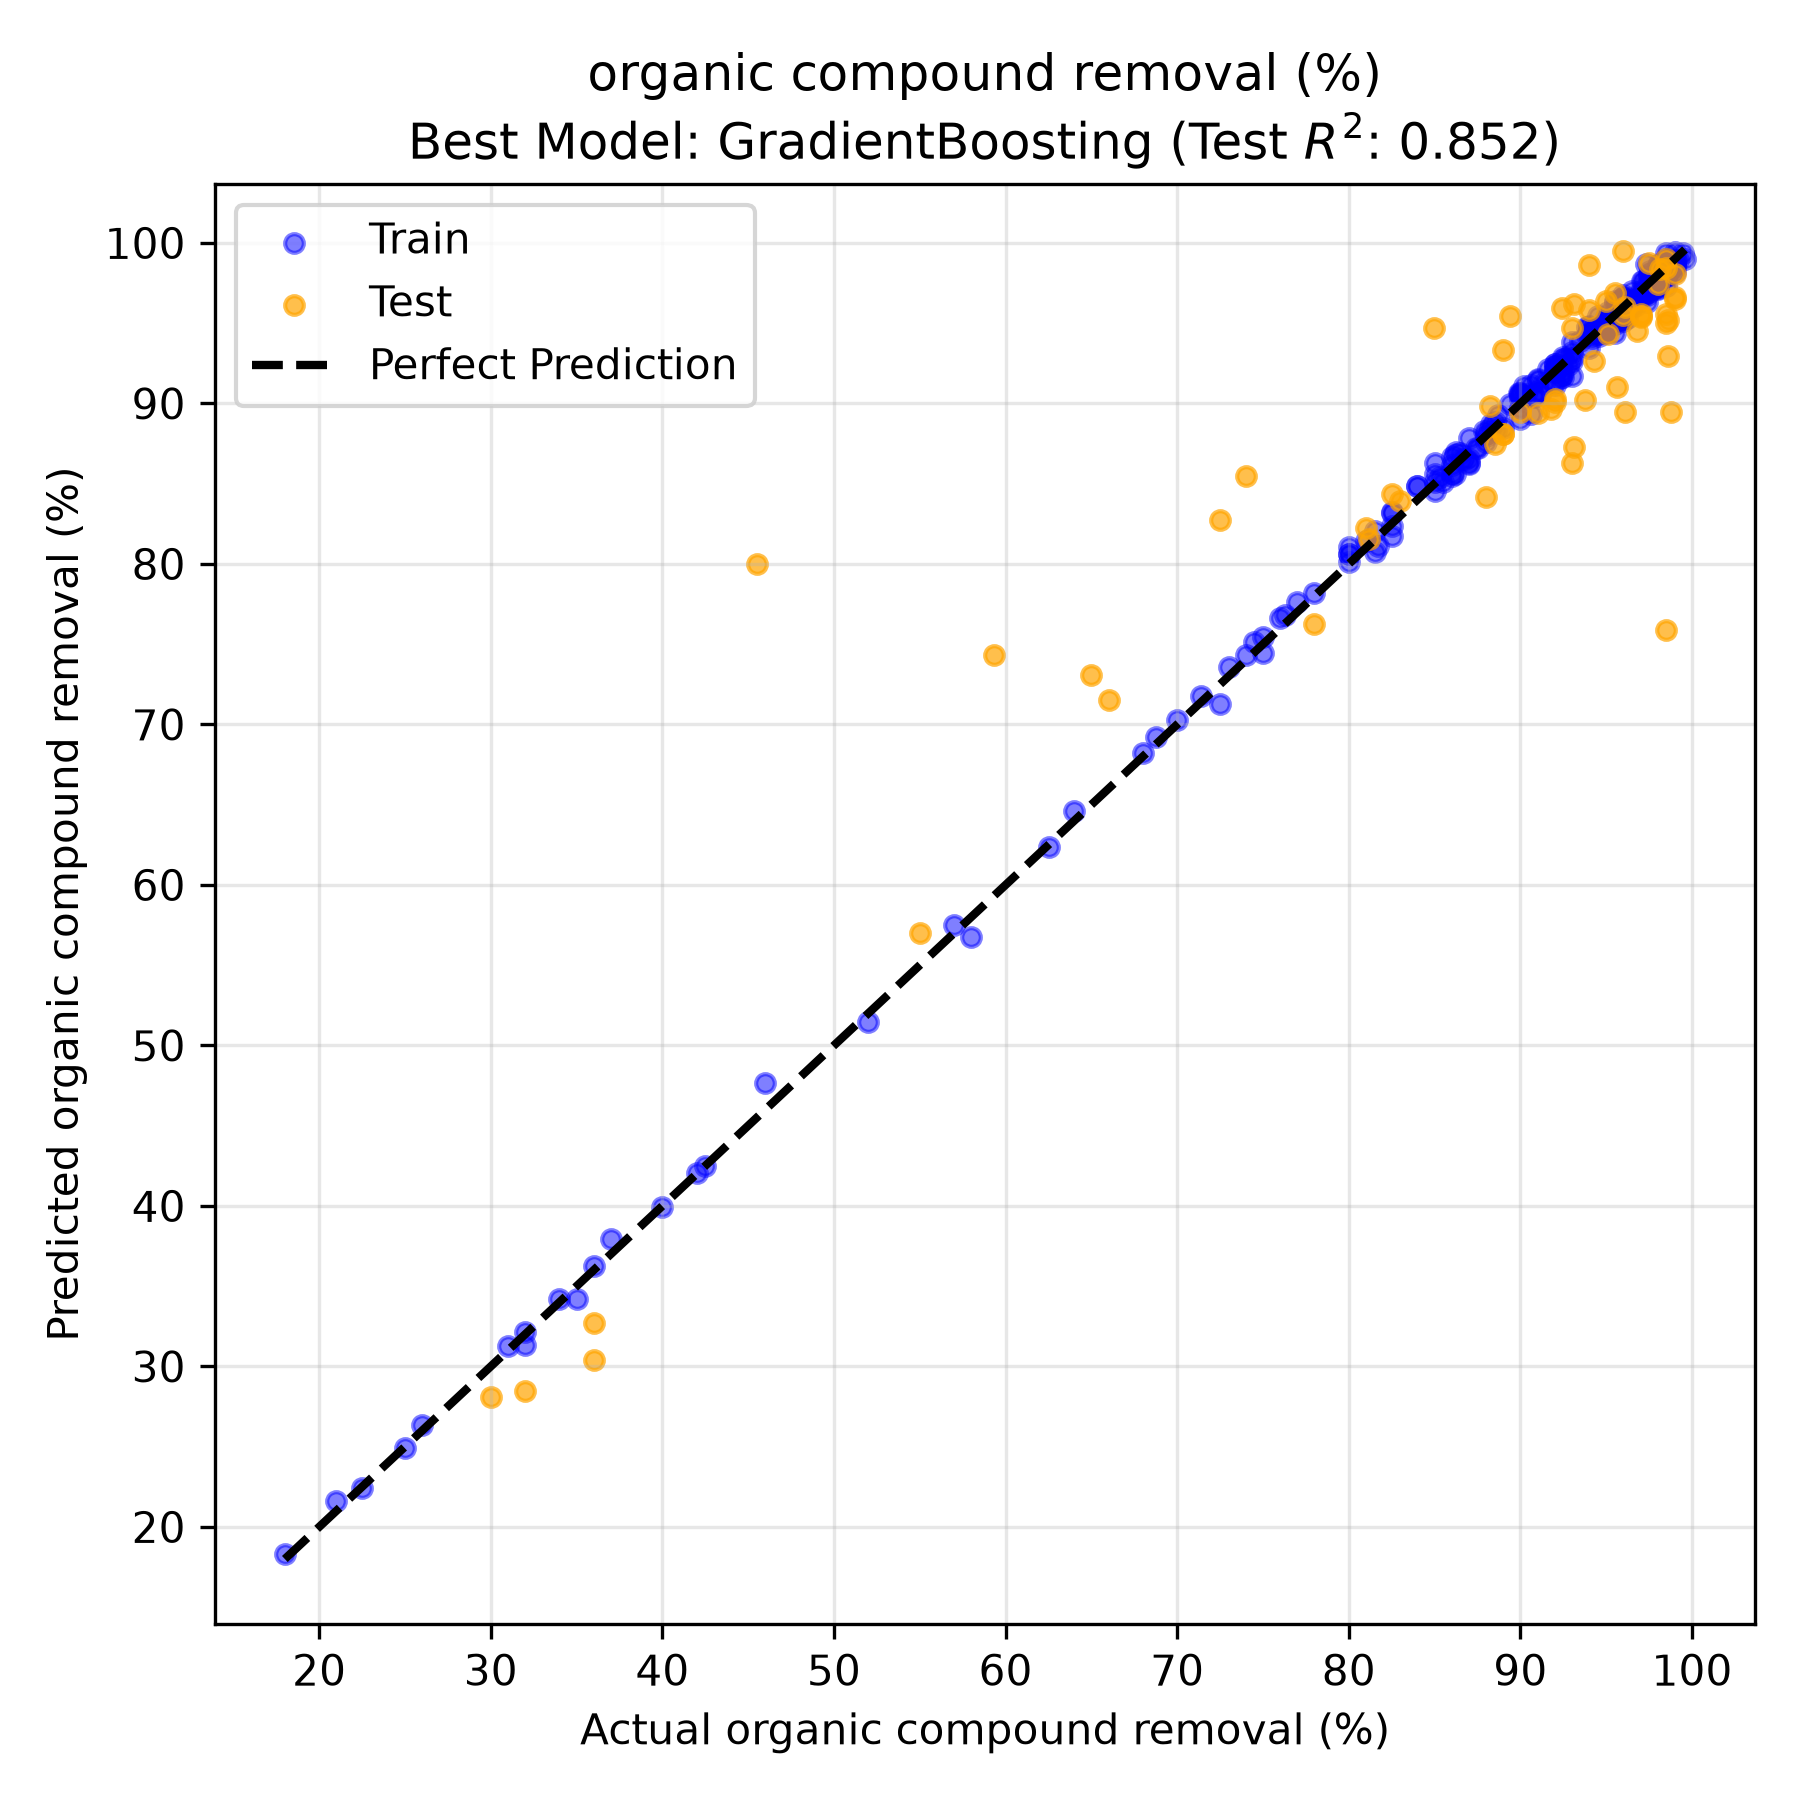
\includegraphics[width=\textwidth]{figures/parity_organic_compound_removal__.png}
\end{minipage}

\vspace{0.5em}
\begin{minipage}{0.48\textwidth}
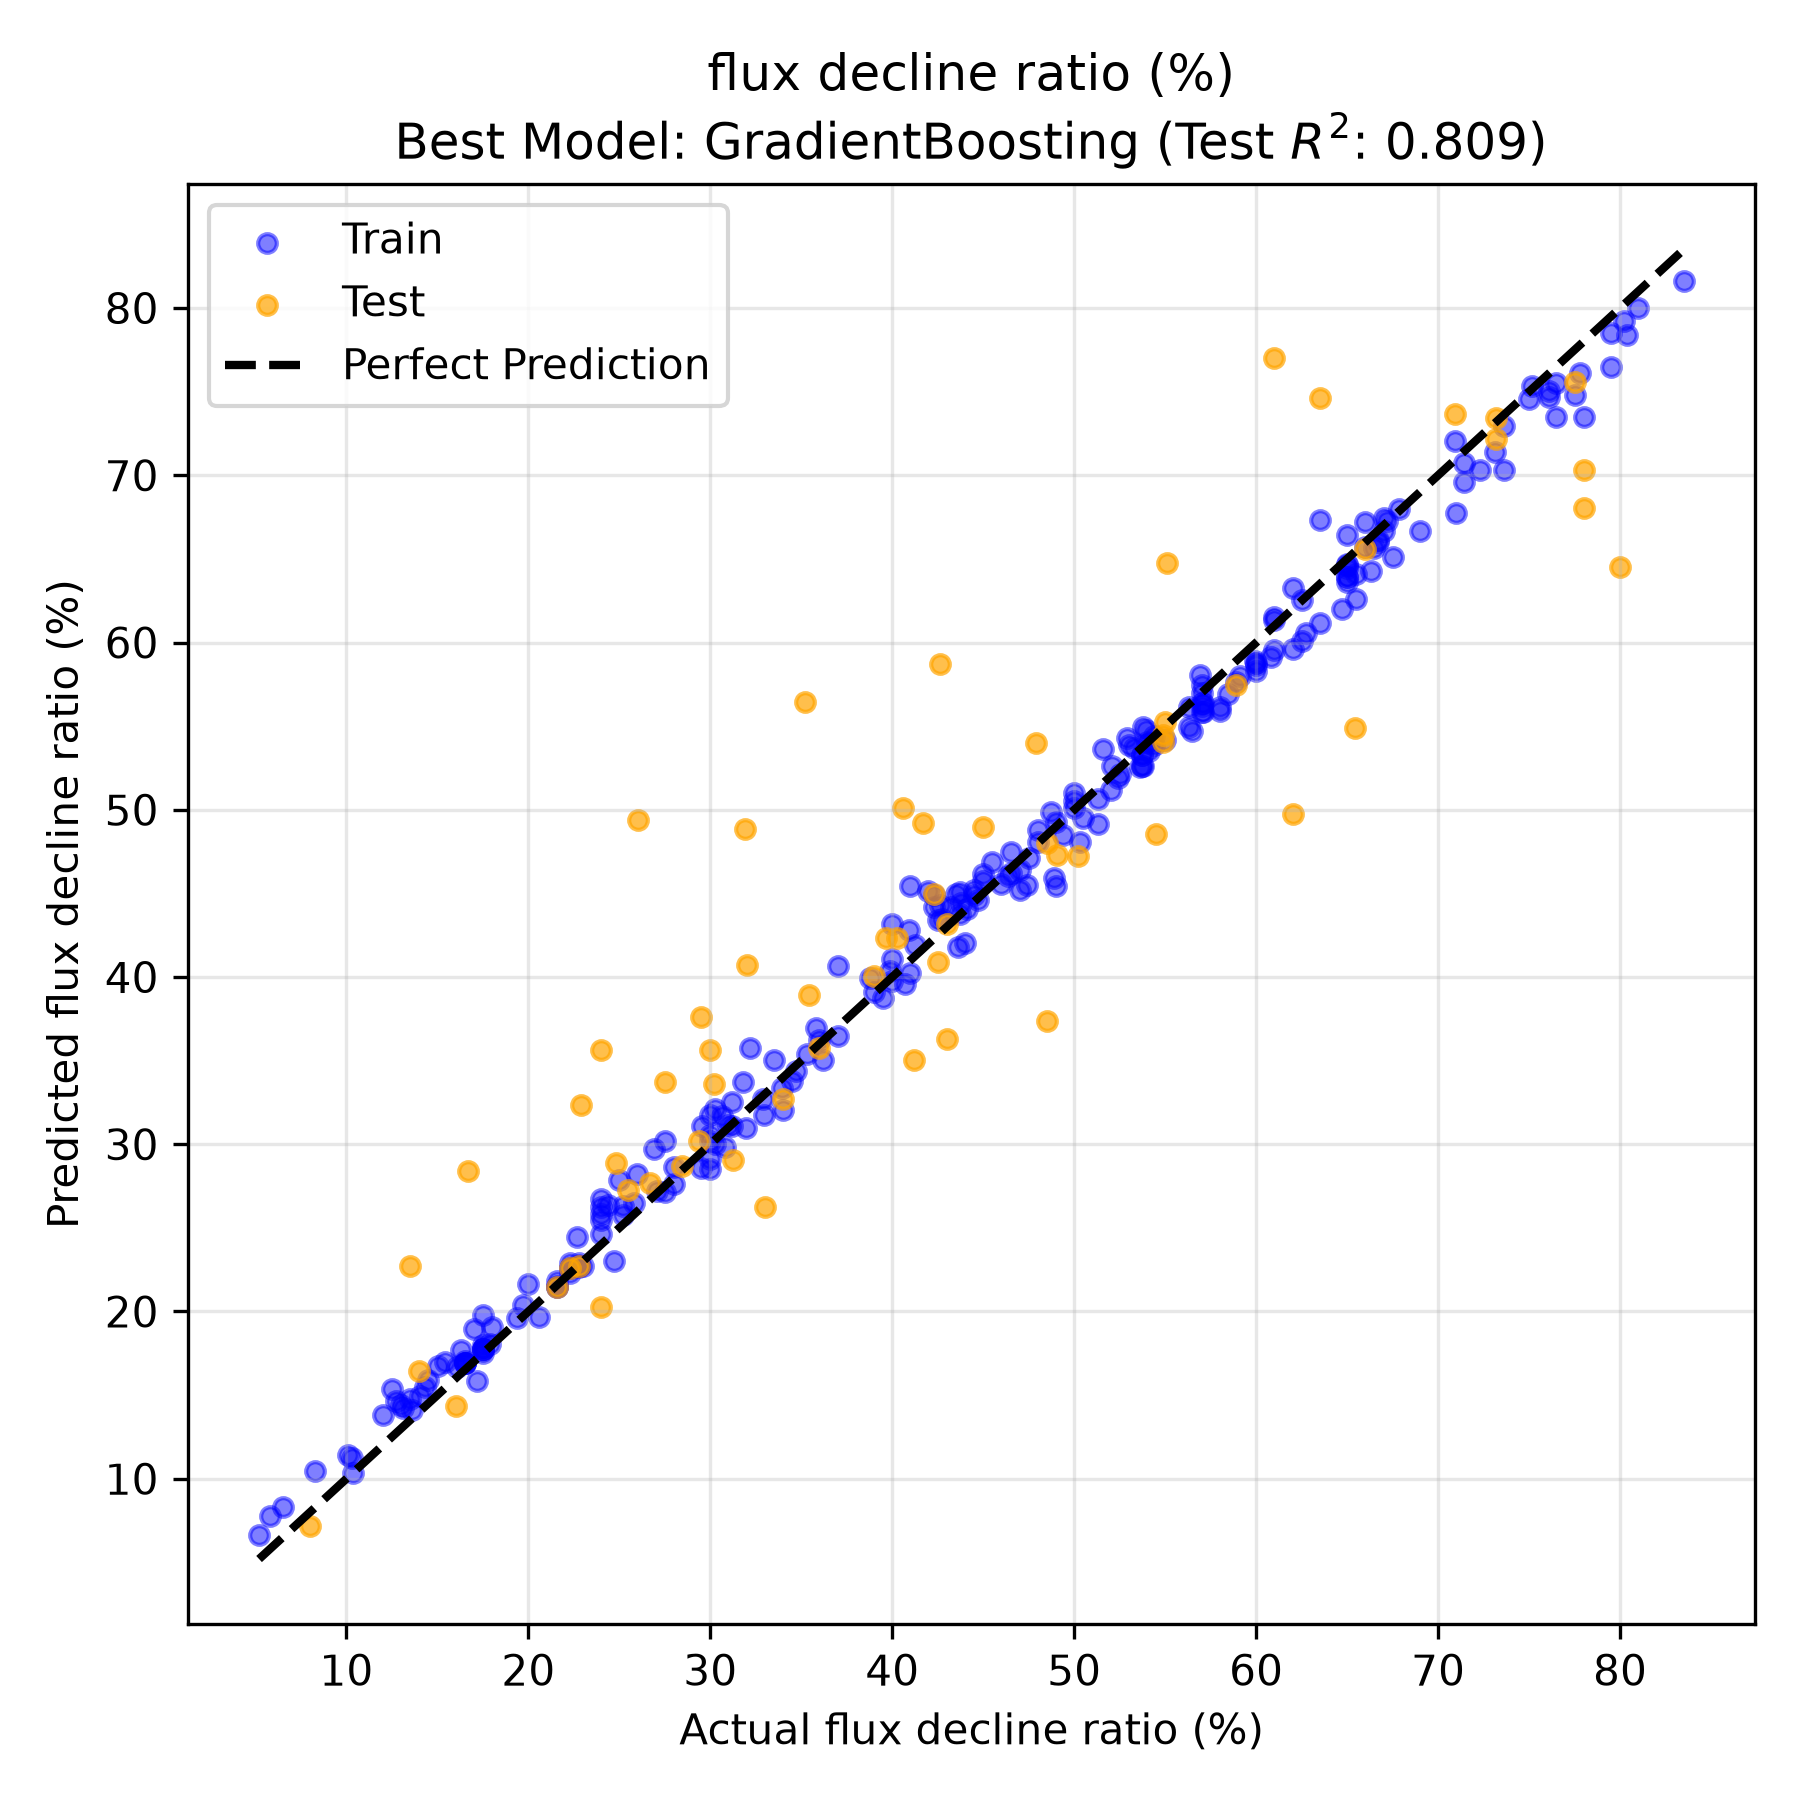
\includegraphics[width=\textwidth]{figures/parity_flux_decline_ratio__.png}
\end{minipage}
\hfill
\begin{minipage}{0.48\textwidth}
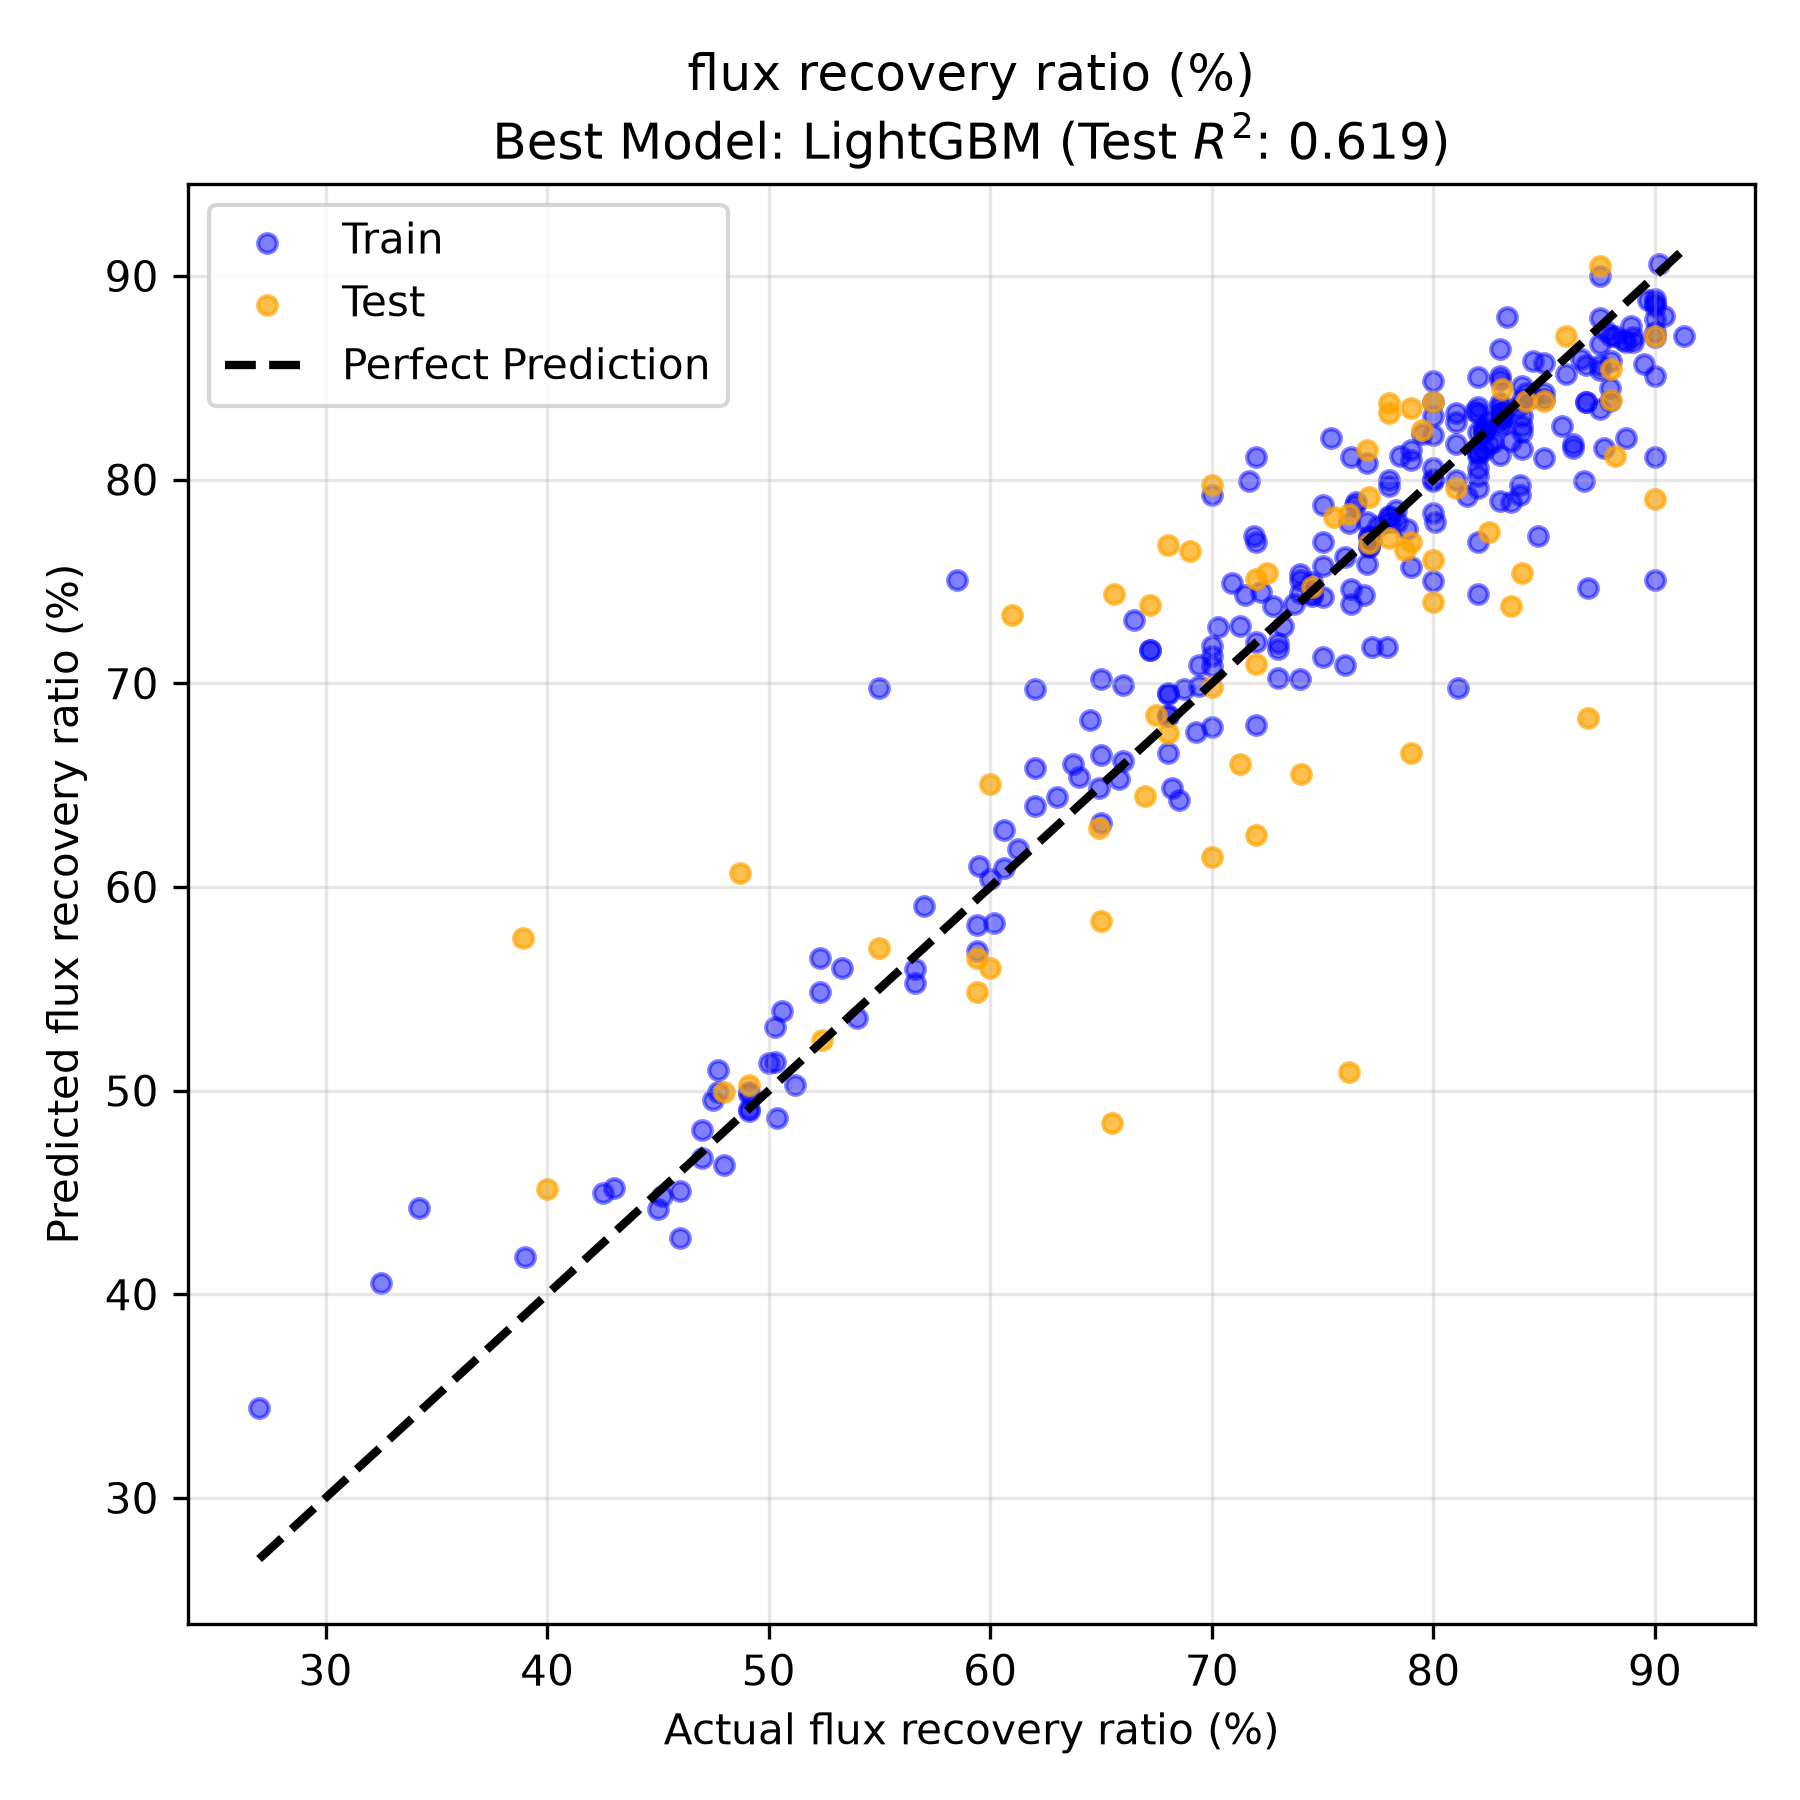
\includegraphics[width=\textwidth]{figures/parity_flux_recovery_ratio__.png}
\end{minipage}

\vspace{0.5em}
\begin{minipage}{0.48\textwidth}
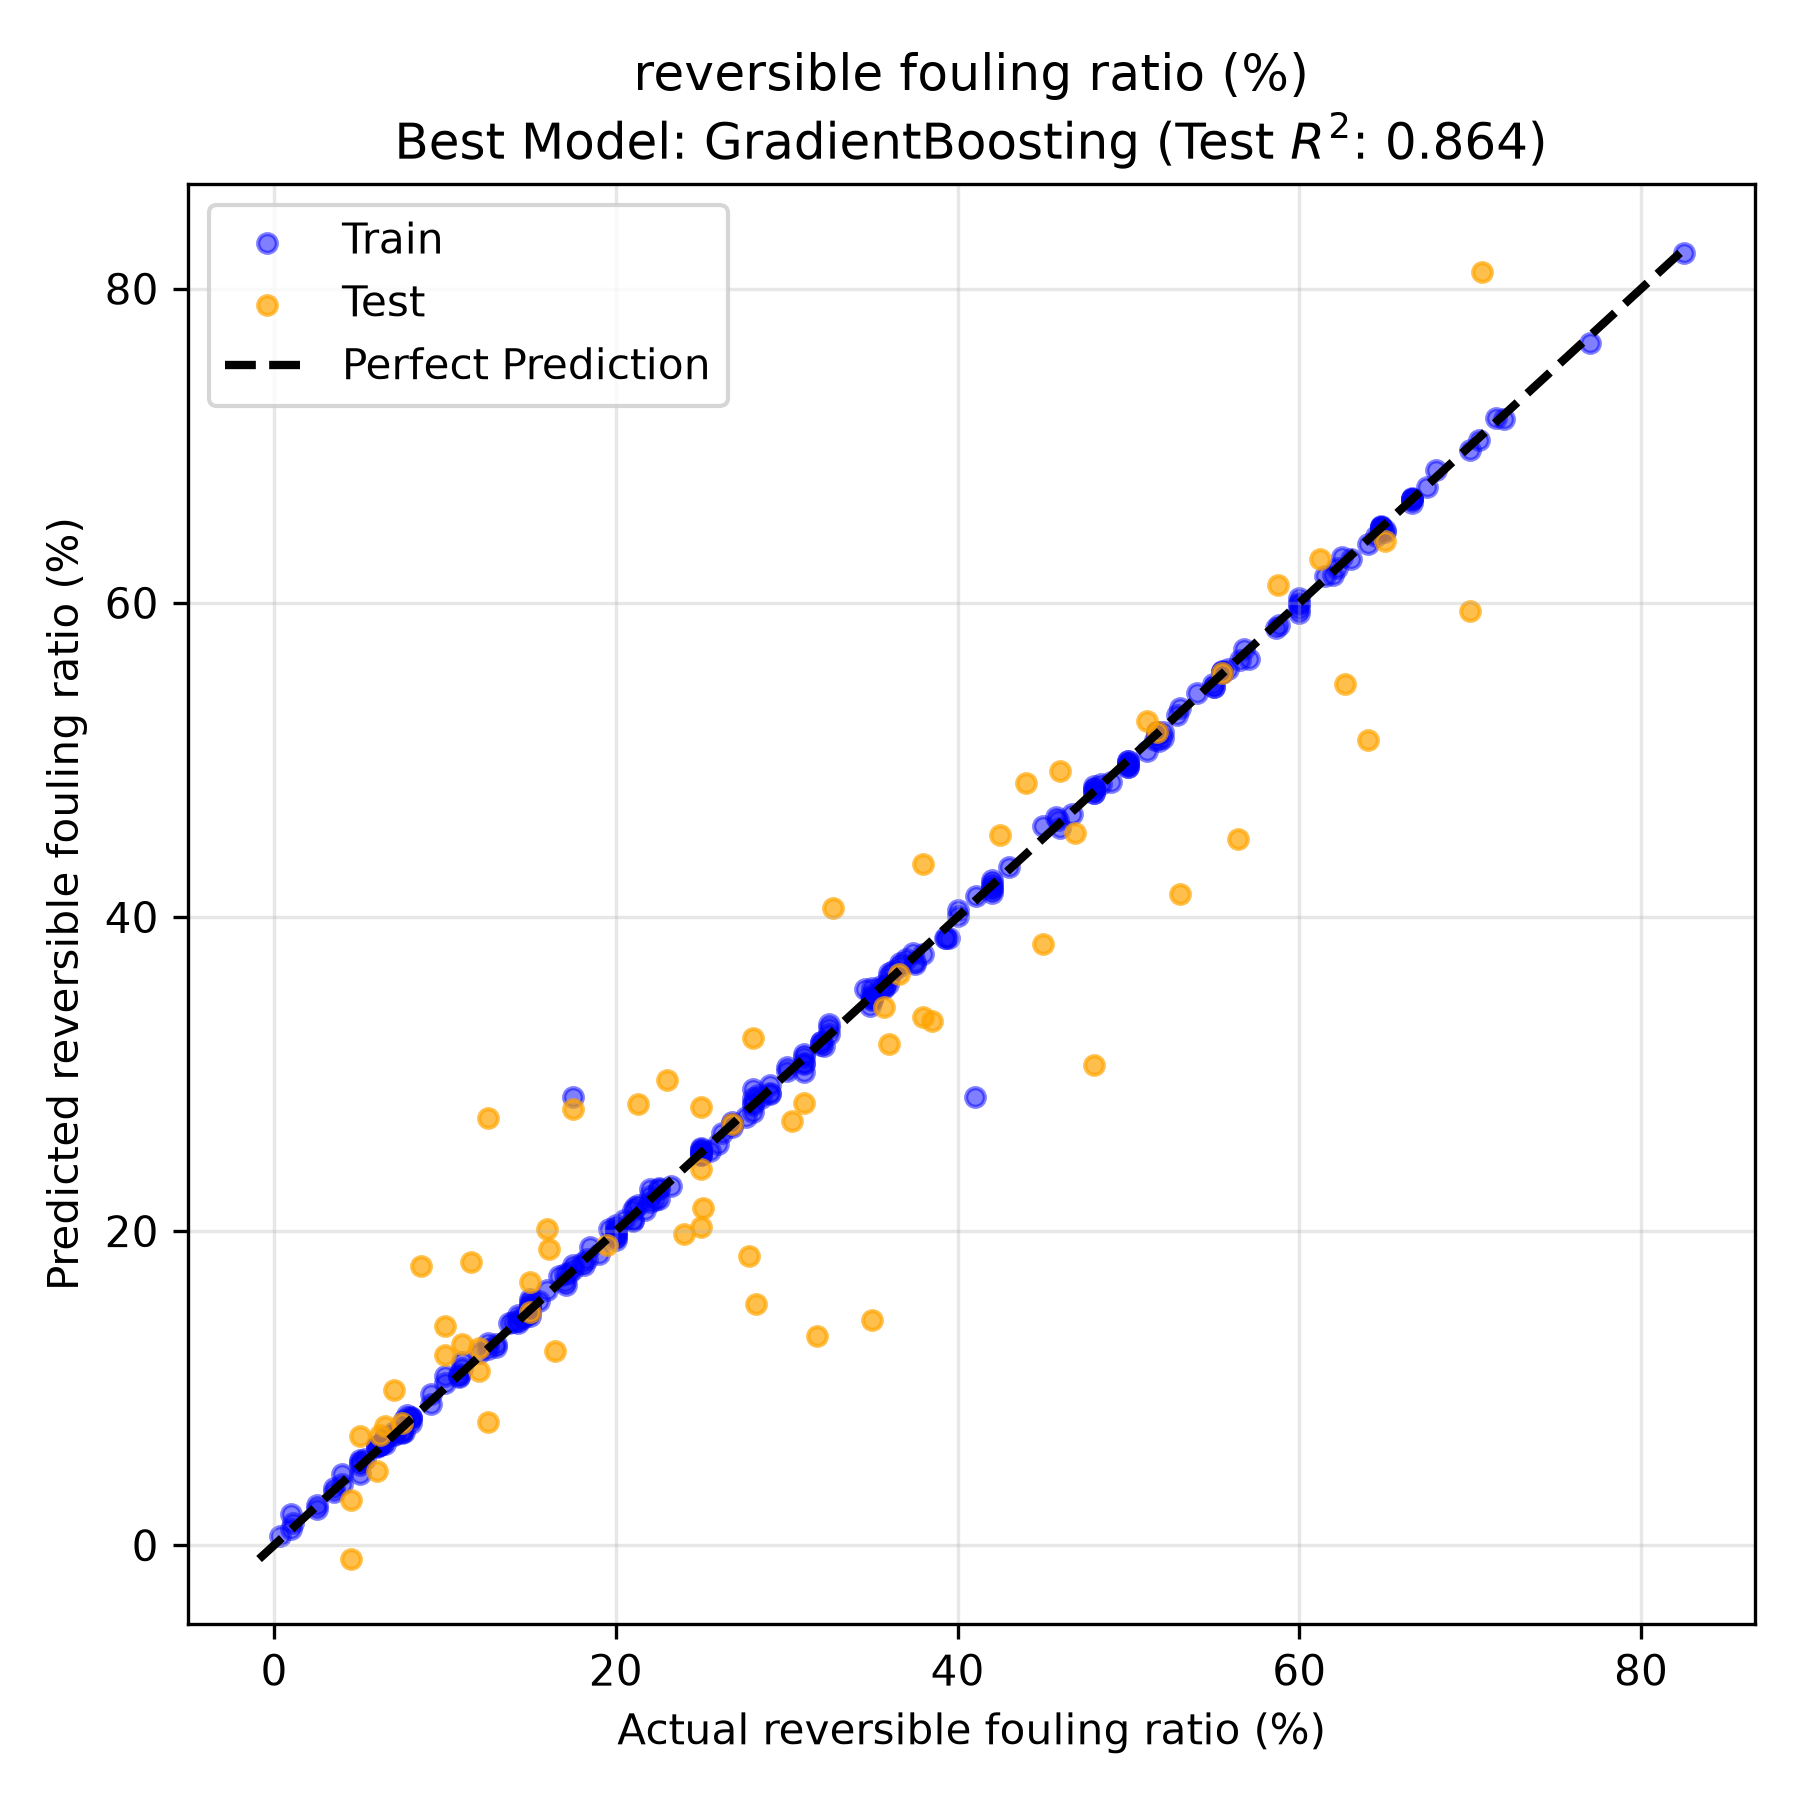
\includegraphics[width=\textwidth]{figures/parity_reversible_fouling_ratio__.png}
\end{minipage}
\caption{Predicted vs.\ actual parity plots (train and test) for each membrane performance target, with the best single model and its test $R^2$ from the parity-plot sweep annotated on each panel. Note the flux recovery ratio panel's annotated model/$R^2$ is the value flagged as an unresolved discrepancy in the text; Table~\ref{tab:performance} retains the higher, previously verified HistGradientBoosting result.}
\label{fig:parity-performance}
\end{figure}

\subsection{Predictive ML Models for Membrane Properties}

Models were also developed to predict three major membrane performance-determining properties using fabrication conditions as input features (Table~\ref{tab:properties}; parity plots in Figure~\ref{fig:parity-properties}). Following the discrepancy resolution in Section 3.1, all three property targets now use Gradient-Boosting-based models. For mean pore radius, the parity-plot sweep's best single model is Kernel Ridge Regression at test $R^2 = 0.810$, essentially matching the previously reported weighted ensemble of Kernel Ridge Regression and RandomForest at $R^2 = 0.826$ (vs.\ $0.809$ with the earlier ExtraTrees + LightGBM ensemble); the ensemble value is retained in Table~\ref{tab:properties} as the better of the two. This narrows, but does not close, the gap to the benchmark ($0.87$) -- the only target of the eight that remains behind benchmark on $R^2$.

For overall porosity, the solo tuned Gradient Boosting model achieved a test $R^2$ of $0.717$ (vs.\ $0.66$), confirmed by the parity plot, beating the benchmark; the corresponding two-model ensemble (GradientBoosting + Kernel Ridge Regression) underperformed the solo model at $R^2 = 0.697$ and is not used. For contact angle, the parity plot confirms the solo tuned Gradient Boosting model at test $R^2 = 0.803$, with the previously reported Gradient-Boosting-containing ensemble (GradientBoosting + Kernel Ridge Regression) marginally ahead at $R^2 = 0.806$ and retained as the reported best; both beat the benchmark ($0.76$) and both replace the earlier multi-task ExtraTrees result ($R^2 = 0.728$). Train-set metrics and RMSE were not captured alongside the parity plots for any of the three property targets and are marked N/R in Table~\ref{tab:properties}.

\begin{table}[htbp]
\centering
\caption{Prediction Performance of the ML Models for Membrane Properties}
\label{tab:properties}
\resizebox{\textwidth}{!}{%
\begin{tabular}{@{}lccccccccc@{}}
\toprule
\multirow{2}{*}{Membrane property} & \multirow{2}{*}{\shortstack{Total\\data size}} & \multicolumn{2}{c}{Train $R^2$} & \multicolumn{2}{c}{Train RMSE} & \multicolumn{2}{c}{Test $R^2$} & \multicolumn{2}{c}{Test RMSE} \\
\cmidrule(lr){3-4}\cmidrule(lr){5-6}\cmidrule(lr){7-8}\cmidrule(lr){9-10}
 & & Gao & Proposed & Gao & Proposed & Gao & Proposed & Gao & Proposed \\
\midrule
Overall porosity (\%) & 320 & 0.96 & N/R   & 2.51 & N/R & 0.66 & \textbf{0.717} & 7.61 & N/R           \\
Mean pore radius (nm) & 320 & 0.98 & N/R   & 3.47 & N/R & 0.87 & 0.826          & 7.59 & N/R           \\
Contact angle (deg)   & 320 & 0.98 & N/R   & 1.87 & N/R & 0.76 & \textbf{0.806} & 5.87 & N/R           \\
\bottomrule
\end{tabular}%
}
\vspace{0.3em}
\begin{flushleft}
\footnotesize \textbf{Bold} indicates the proposed solution beats the Gao et al.\ benchmark for that specific metric. N/R = not reported in the current tuning round.
\end{flushleft}
\end{table}

\begin{figure}[htbp]
\centering
\begin{minipage}{0.48\textwidth}
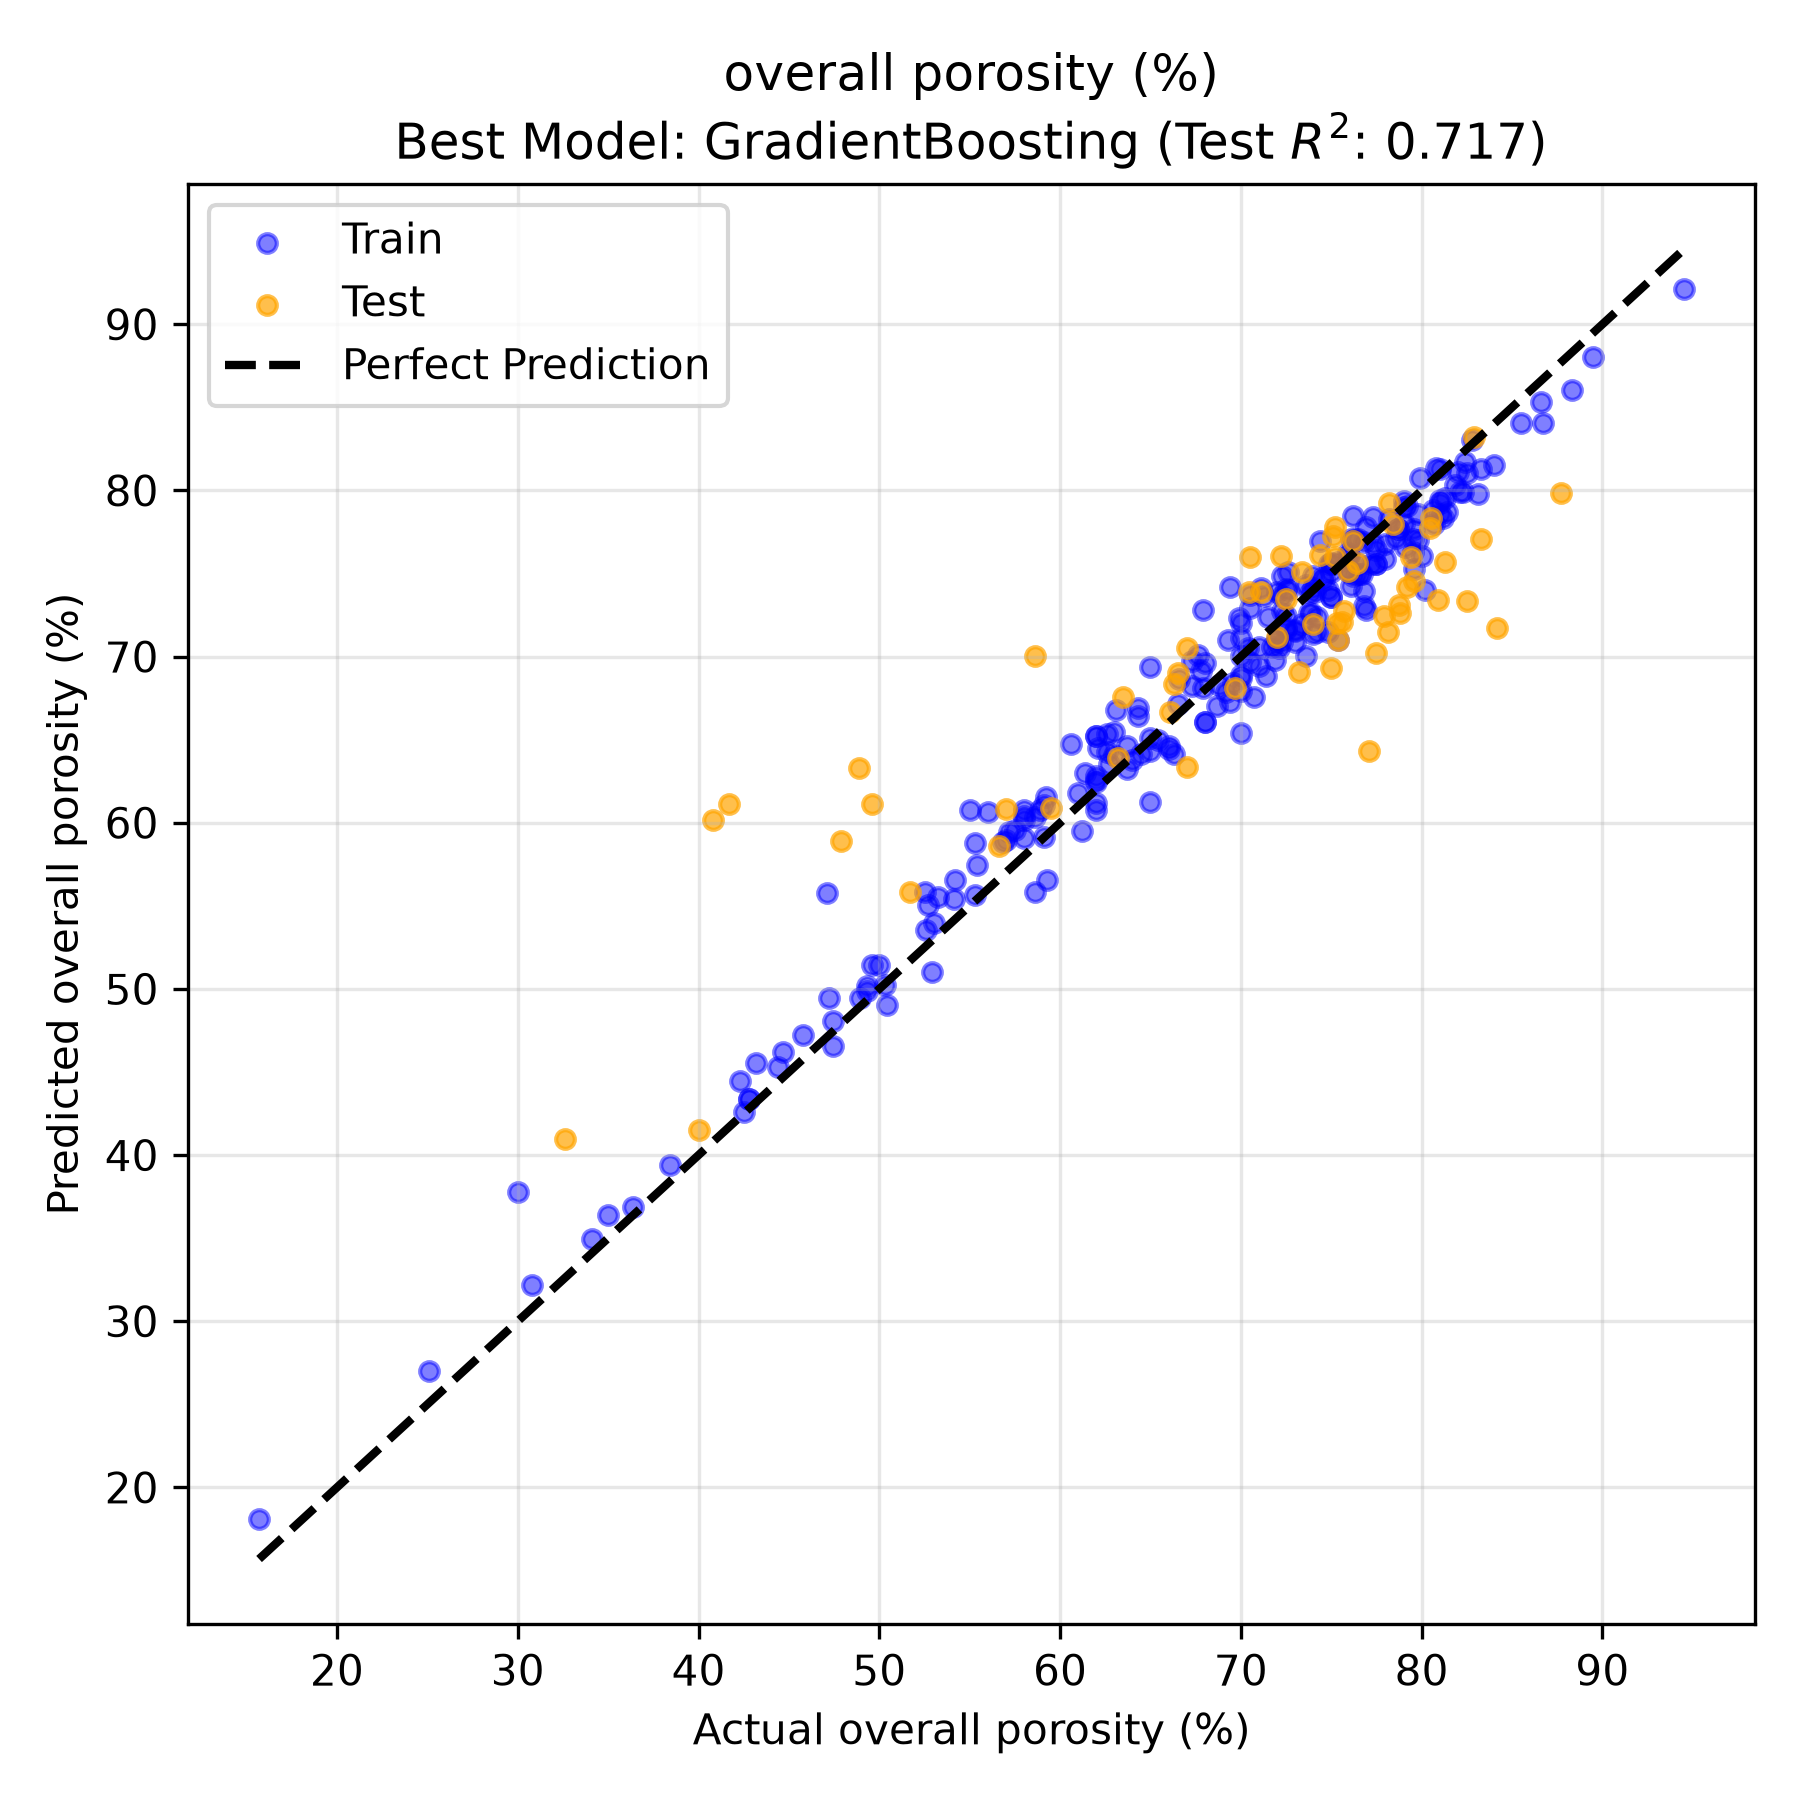
\includegraphics[width=\textwidth]{figures/parity_overall_porosity__.png}
\end{minipage}
\hfill
\begin{minipage}{0.48\textwidth}
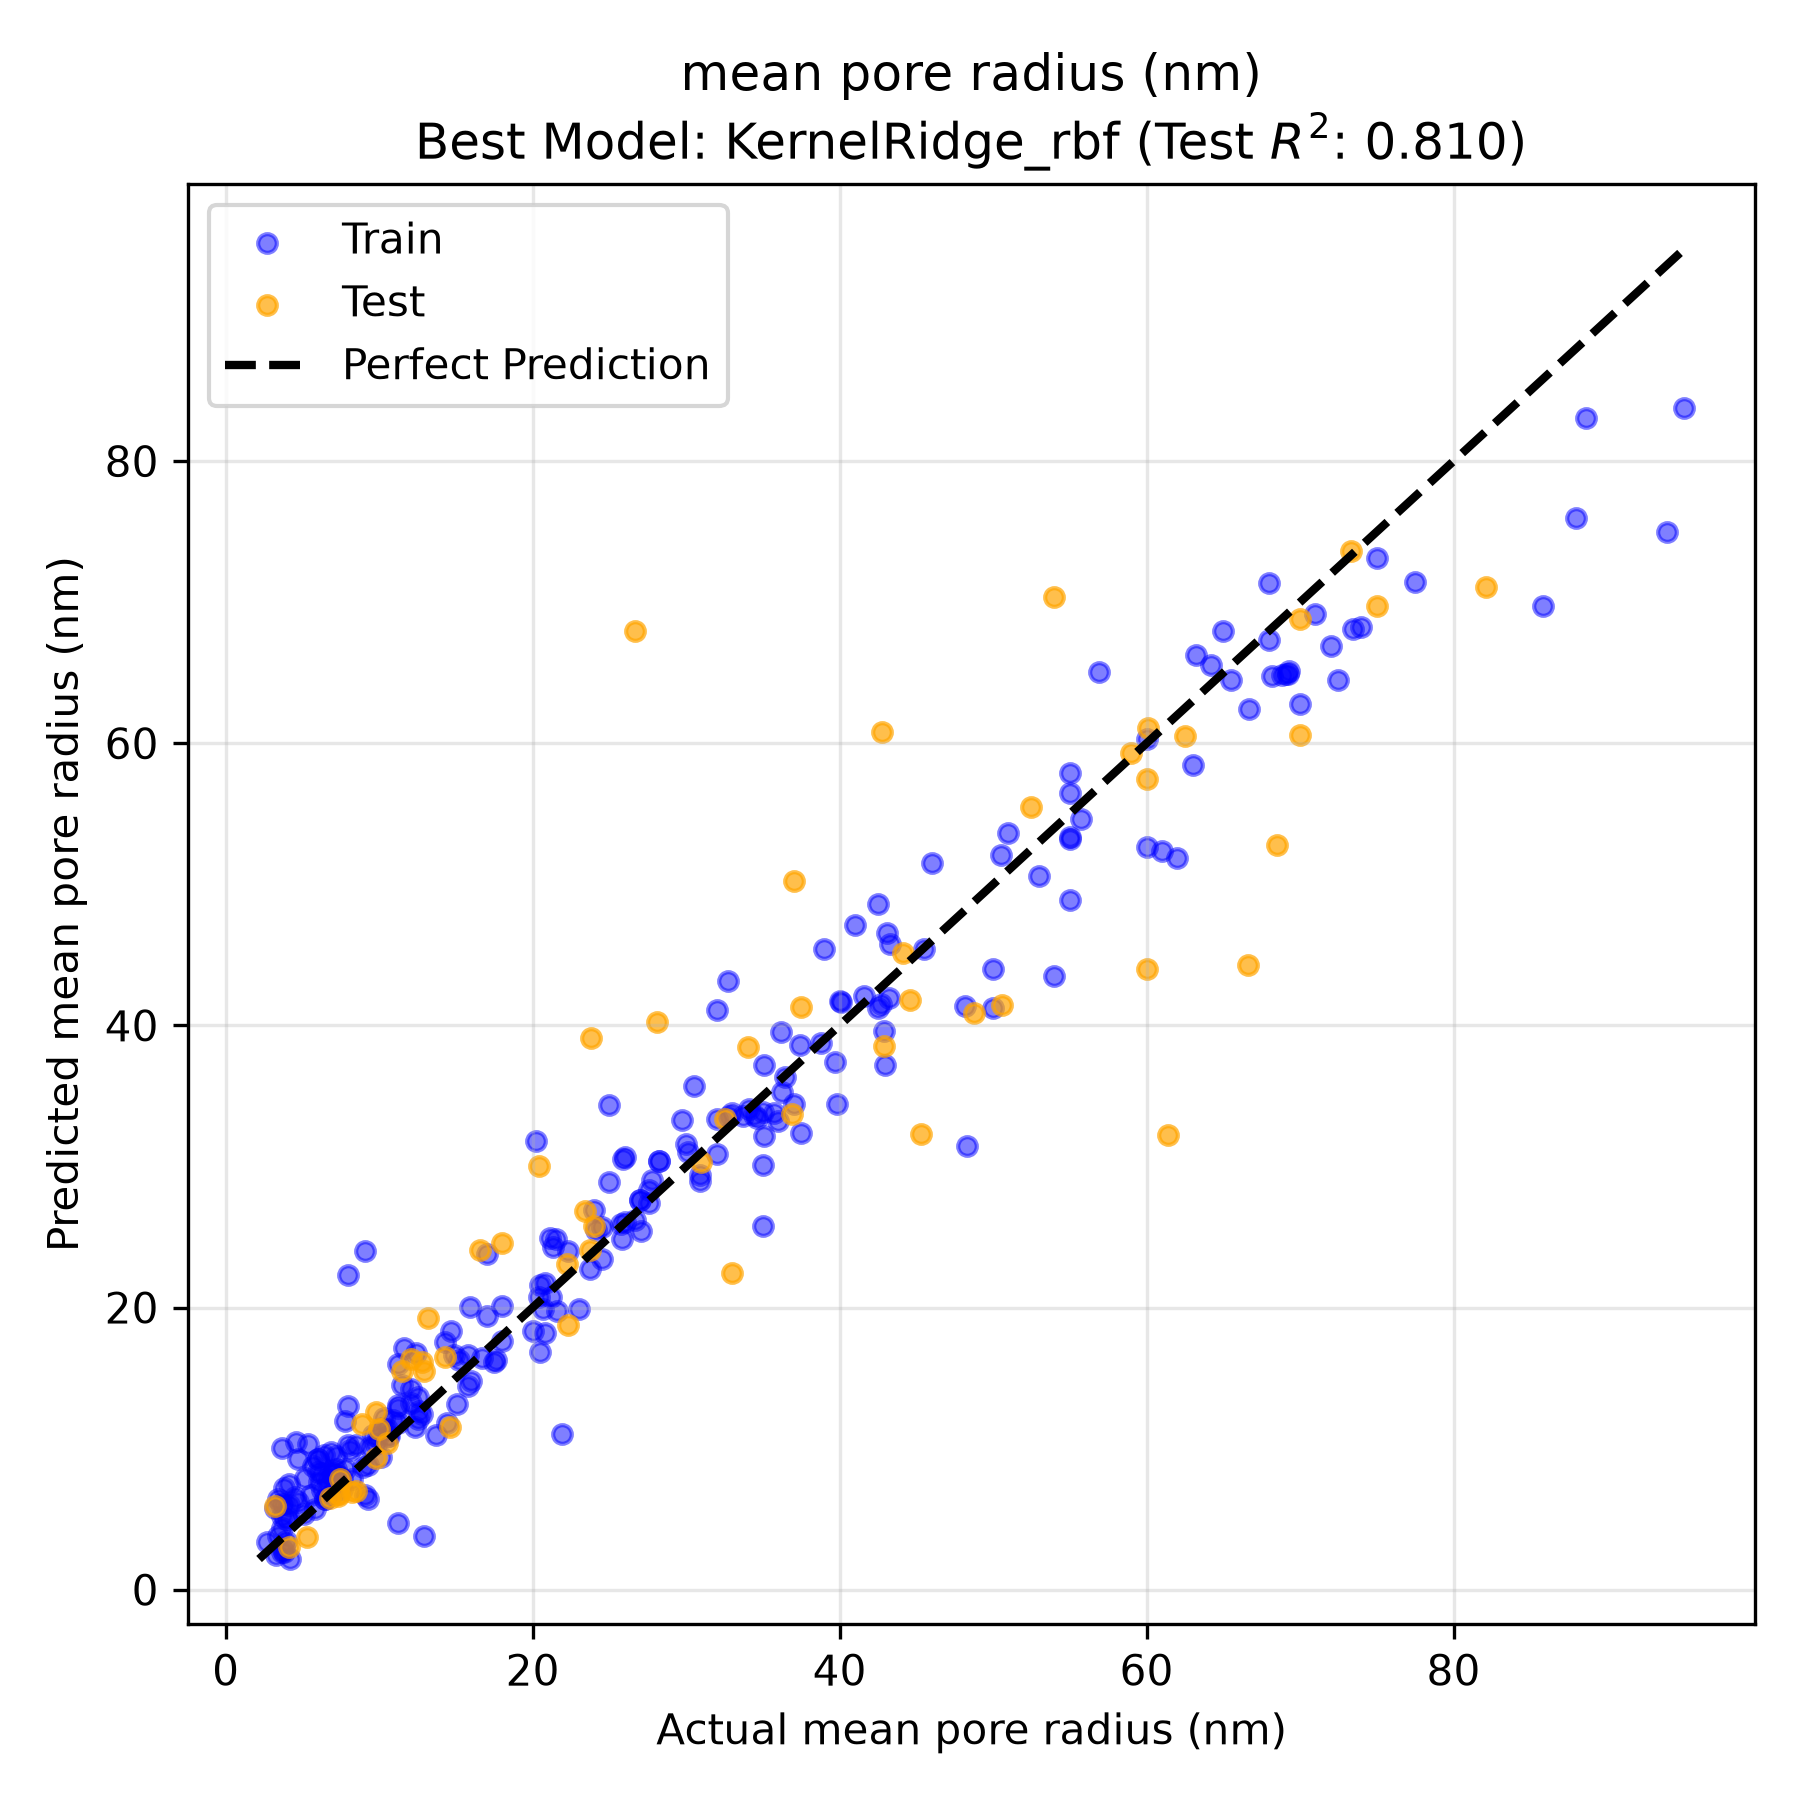
\includegraphics[width=\textwidth]{figures/parity_mean_pore_radius_nm.png}
\end{minipage}

\vspace{0.5em}
\begin{minipage}{0.48\textwidth}
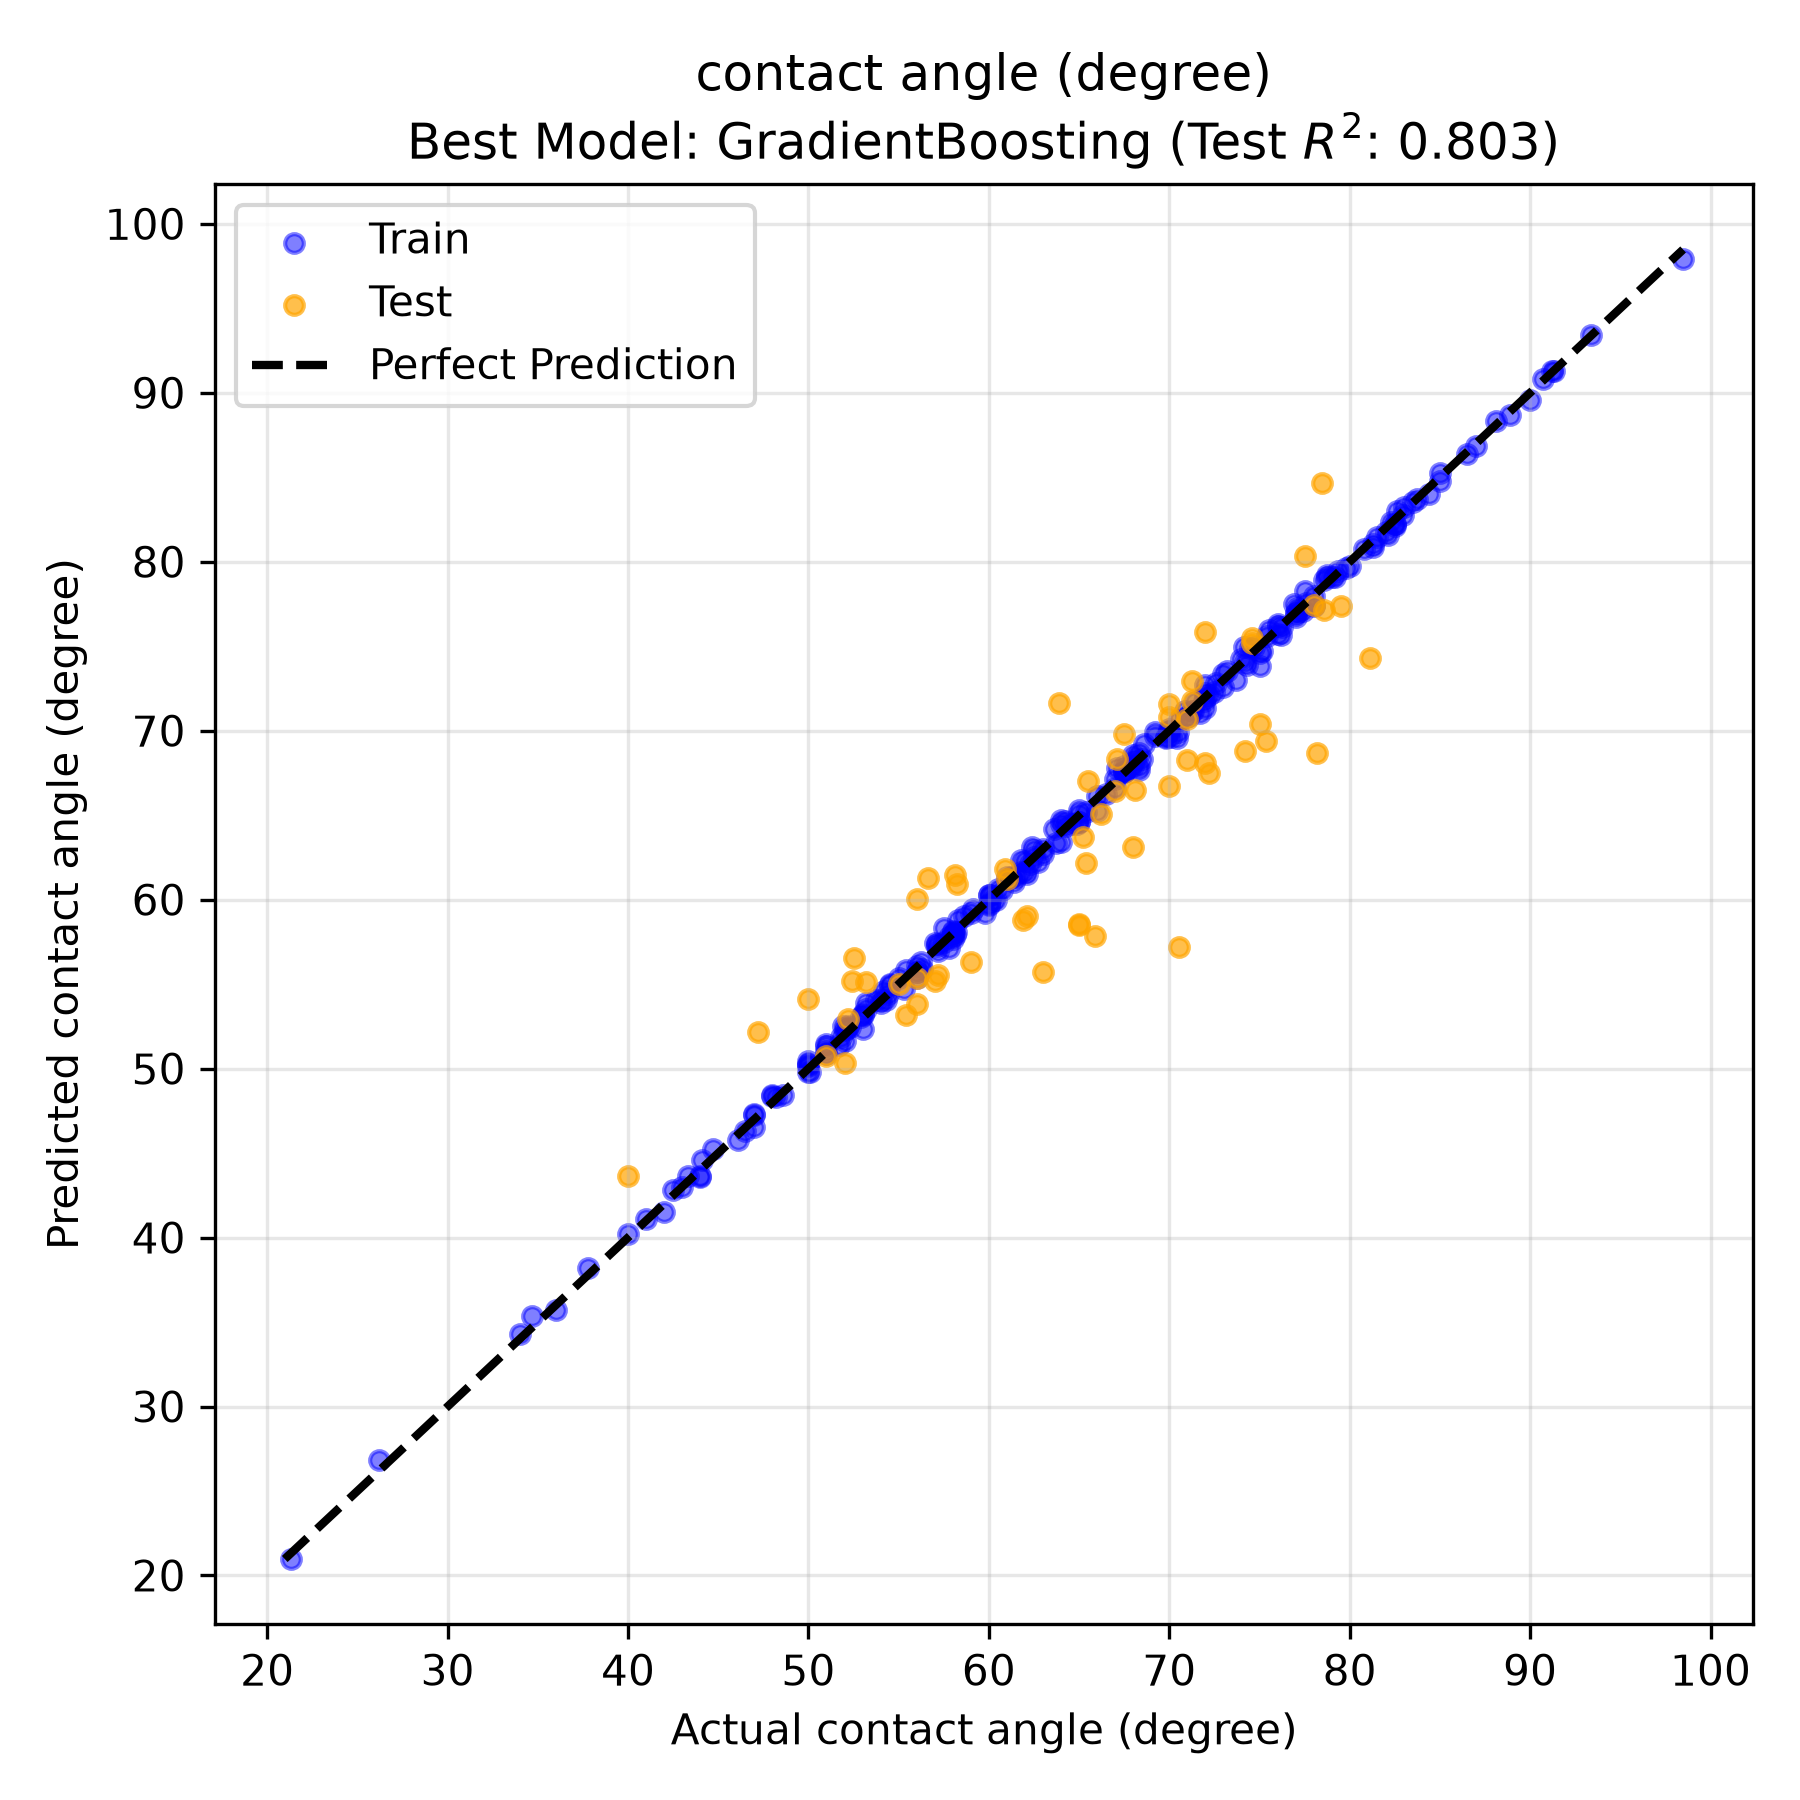
\includegraphics[width=\textwidth]{figures/parity_contact_angle_degree.png}
\end{minipage}
\caption{Predicted vs.\ actual parity plots (train and test) for each membrane property target, with the best single model and its test $R^2$ from the parity-plot sweep annotated on each panel. For mean pore radius and contact angle, Table~\ref{tab:properties} reports a marginally higher ensemble value than the solo model annotated here (see text).}
\label{fig:parity-properties}
\end{figure}

\subsection{Overfitting, Generalization, and Methodological Limitations}

An analysis of the training versus testing metrics reveals a notable generalization gap for the three performance targets whose train-set metrics remain available from the original tuned zoo (water permeability, flux recovery ratio, reversible fouling ratio). These exhibit training $R^2$ values ranging from $0.914$ to $0.981$, contrasting with test $R^2$ values between $0.638$ and $0.845$. This overfitting gap ($\Delta R^2 \approx 0.06$ to $0.28$) is consistent with the limitations observed in the source paper. Train-set metrics for the five targets updated in the latest tuning round (organic compound removal, flux decline ratio, overall porosity, mean pore radius, contact angle) were not captured during that run and are marked N/R in Tables~\ref{tab:performance} and~\ref{tab:properties}; consequently, whether the newly reported test-$R^2$ gains for those five targets come with a correspondingly larger or smaller overfitting gap cannot currently be assessed, and is flagged as an item to capture in the next tuning pass rather than assumed to match the pattern seen in the three unchanged targets.

A second, more severe generalization concern surfaces under leakage-safe, DOI-grouped 5-fold cross-validation (Section 2.3). This analysis has not been re-run against the newly tuned GradientBoosting-based models, so the numbers below still describe the original 16-model untuned screen. When folds are grouped by source-publication DOI rather than assigned by random row-level split, mean $R^2$ collapses sharply and frequently turns negative across the sixteen-model screen: for example, grouped-CV $R^2$ falls to $-1.30$ for LightGBM on flux decline ratio (versus $0.798$ under the random split) and to $-0.57$ for ExtraTrees on organic compound removal (versus $0.775$ under the random split). Water permeability is the exception, where grouped-CV $R^2$ remains positive for most models but still degrades substantially (e.g., ExtraTrees: $0.846$ random-split vs.\ $0.356$ grouped-CV). This indicates that a non-trivial share of the random-split predictive accuracy reported in Tables~\ref{tab:performance} and~\ref{tab:properties} -- for the proposed solution and, by extension, potentially for the original Gao et al.\ benchmark, which was evaluated under a similar random-split convention -- may partly reflect correlated data points from the same source publication appearing in both the training and test partitions, rather than purely reflecting generalization to unseen membrane fabrication regimes. This is reported here as a limitation to be investigated further rather than as a refutation of the headline results, since the proposed solution and the original benchmark are being compared on the same, matched evaluation convention. Whether the newly tuned GradientBoosting-based models degrade by a similar, larger, or smaller margin under DOI-grouped evaluation is not yet known and is a direct next step.

\begin{figure}[htbp]
\centering
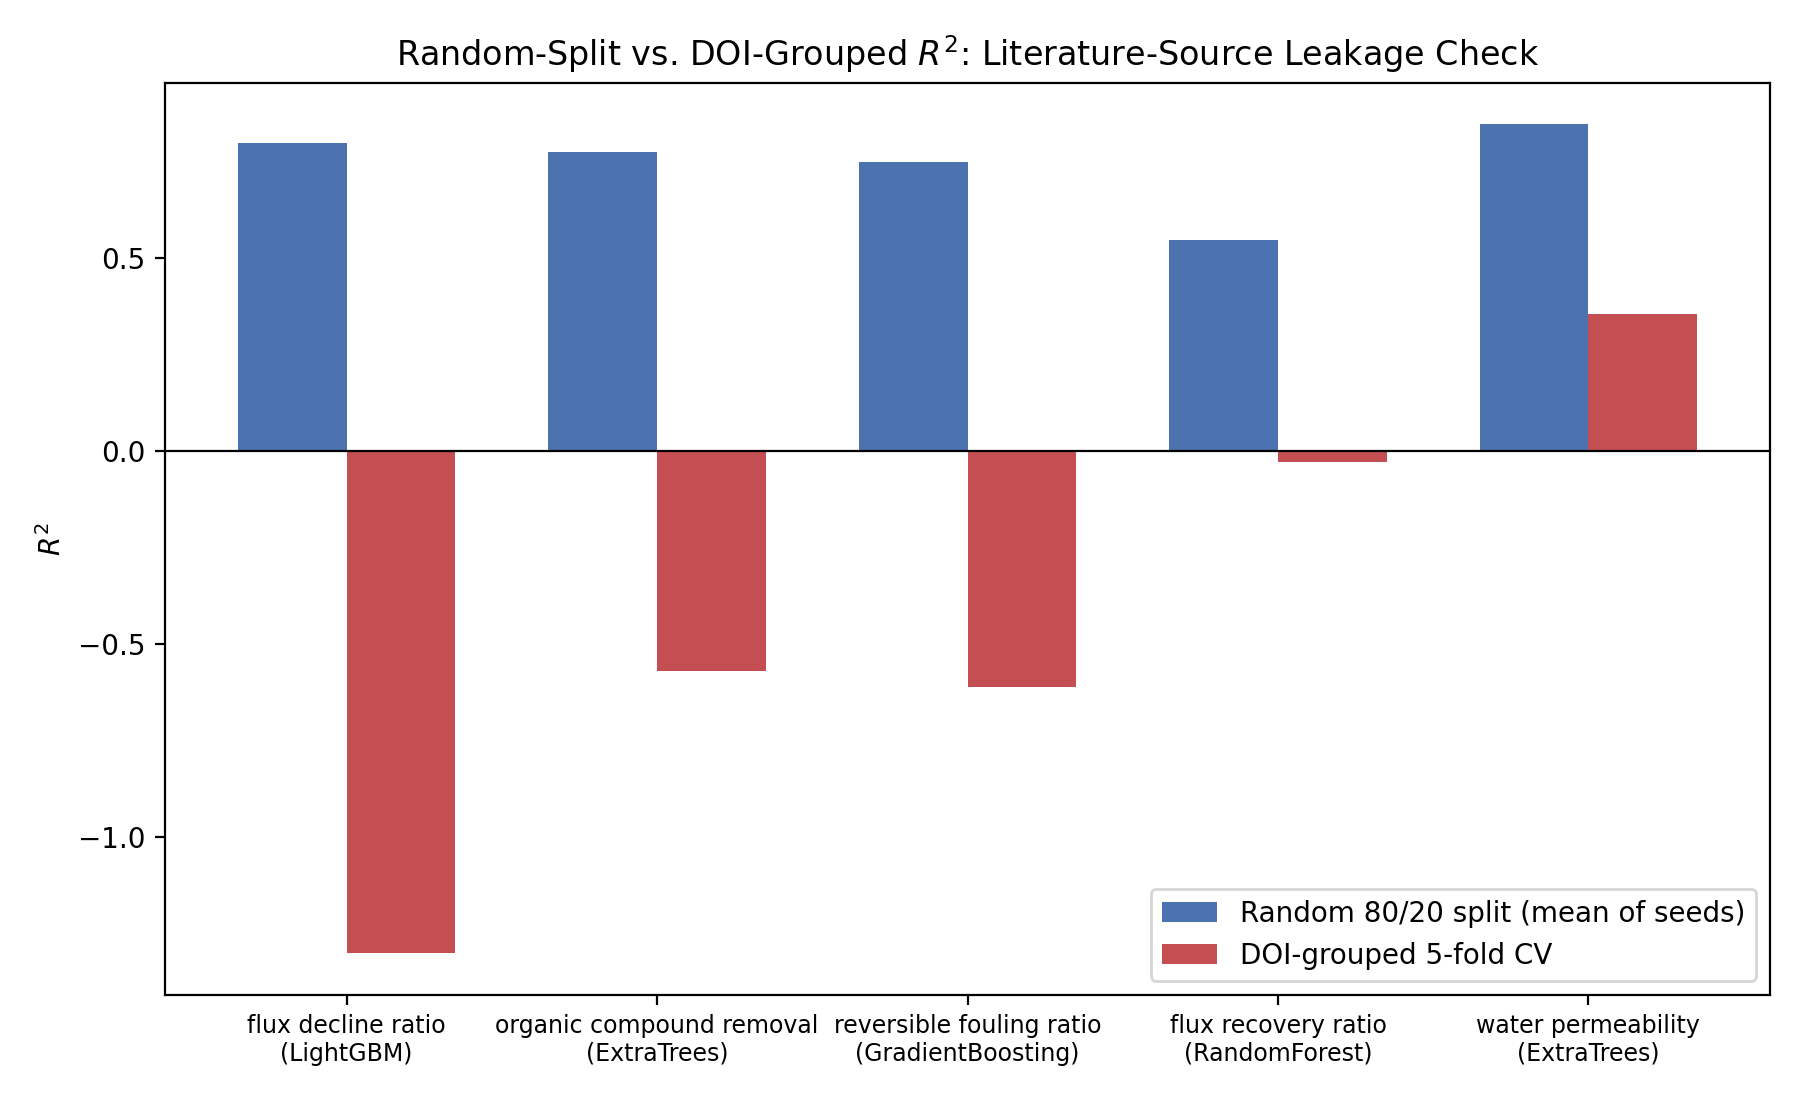
\includegraphics[width=0.85\textwidth]{figures/fig_leakage_comparison.png}
\caption{Mean $R^2$ under the random 80/20 split versus leakage-safe, DOI-grouped 5-fold cross-validation, for the top untuned model on each of five performance targets.}
\label{fig:leakage}
\end{figure}

Figure~\ref{fig:overfitting} illustrates the training-versus-test $R^2$ gap from the original tuned single-model results (seed $= 1000$); note that five of its eight bars (organic compound removal, flux decline ratio, overall porosity, mean pore radius, contact angle) reflect the prior tuning round's models and have not been regenerated for the updated GradientBoosting-based models reported in Tables~\ref{tab:performance} and~\ref{tab:properties}, consistent with the N/R train-metric entries noted above. Figure~\ref{fig:seedvar} shows the seed-to-seed spread underlying the untuned mean $R^2$ values in Table~\ref{tab:baseline}, unaffected by the tuning update.

\begin{figure}[htbp]
\centering
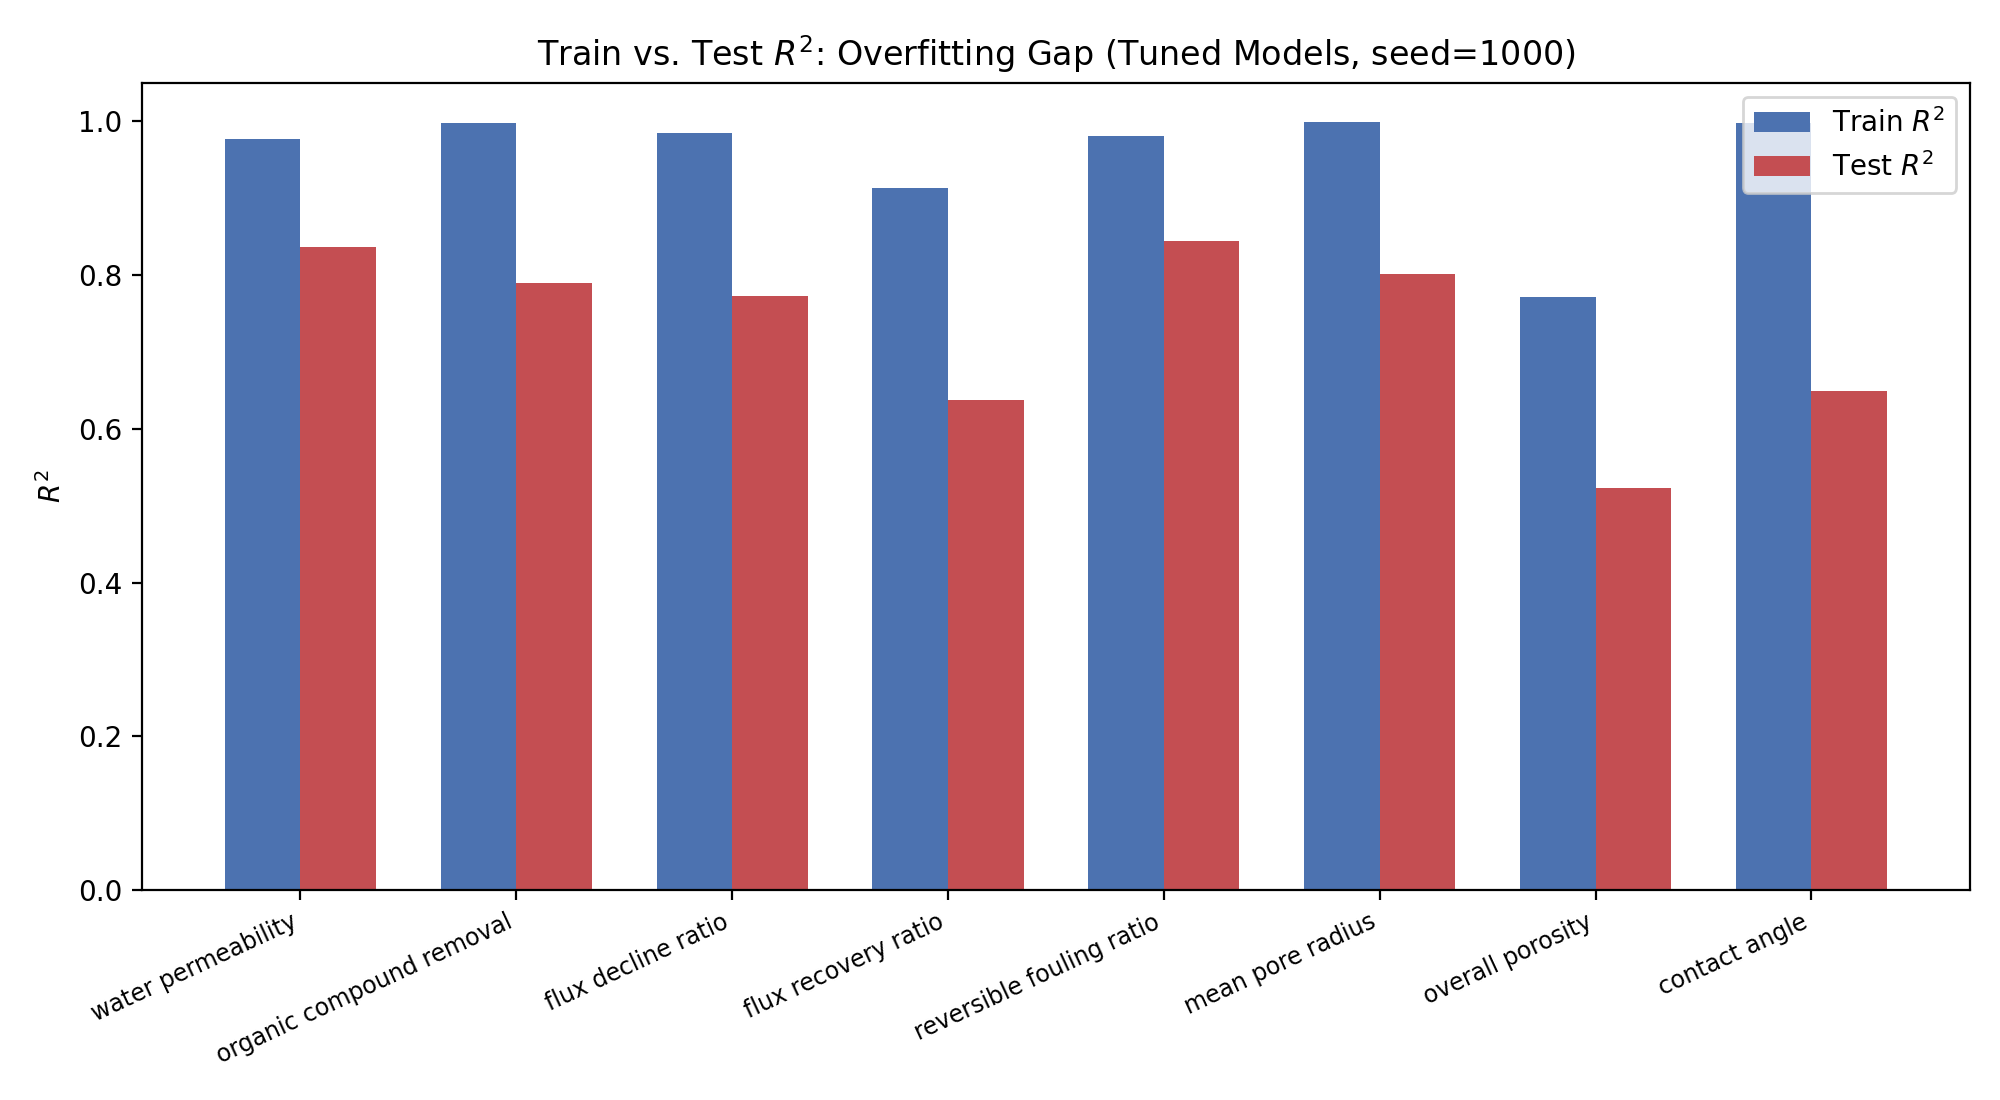
\includegraphics[width=0.85\textwidth]{figures/fig_overfitting_gap.png}
\caption{Train versus test $R^2$ for the tuned single-model results at seed $=1000$. Bars for organic compound removal, flux decline ratio, overall porosity, mean pore radius, and contact angle reflect the prior tuning round's models, superseded in Tables~\ref{tab:performance}--\ref{tab:properties}; only water permeability, flux recovery ratio, and reversible fouling ratio are current.}
\label{fig:overfitting}
\end{figure}

\begin{figure}[htbp]
\centering
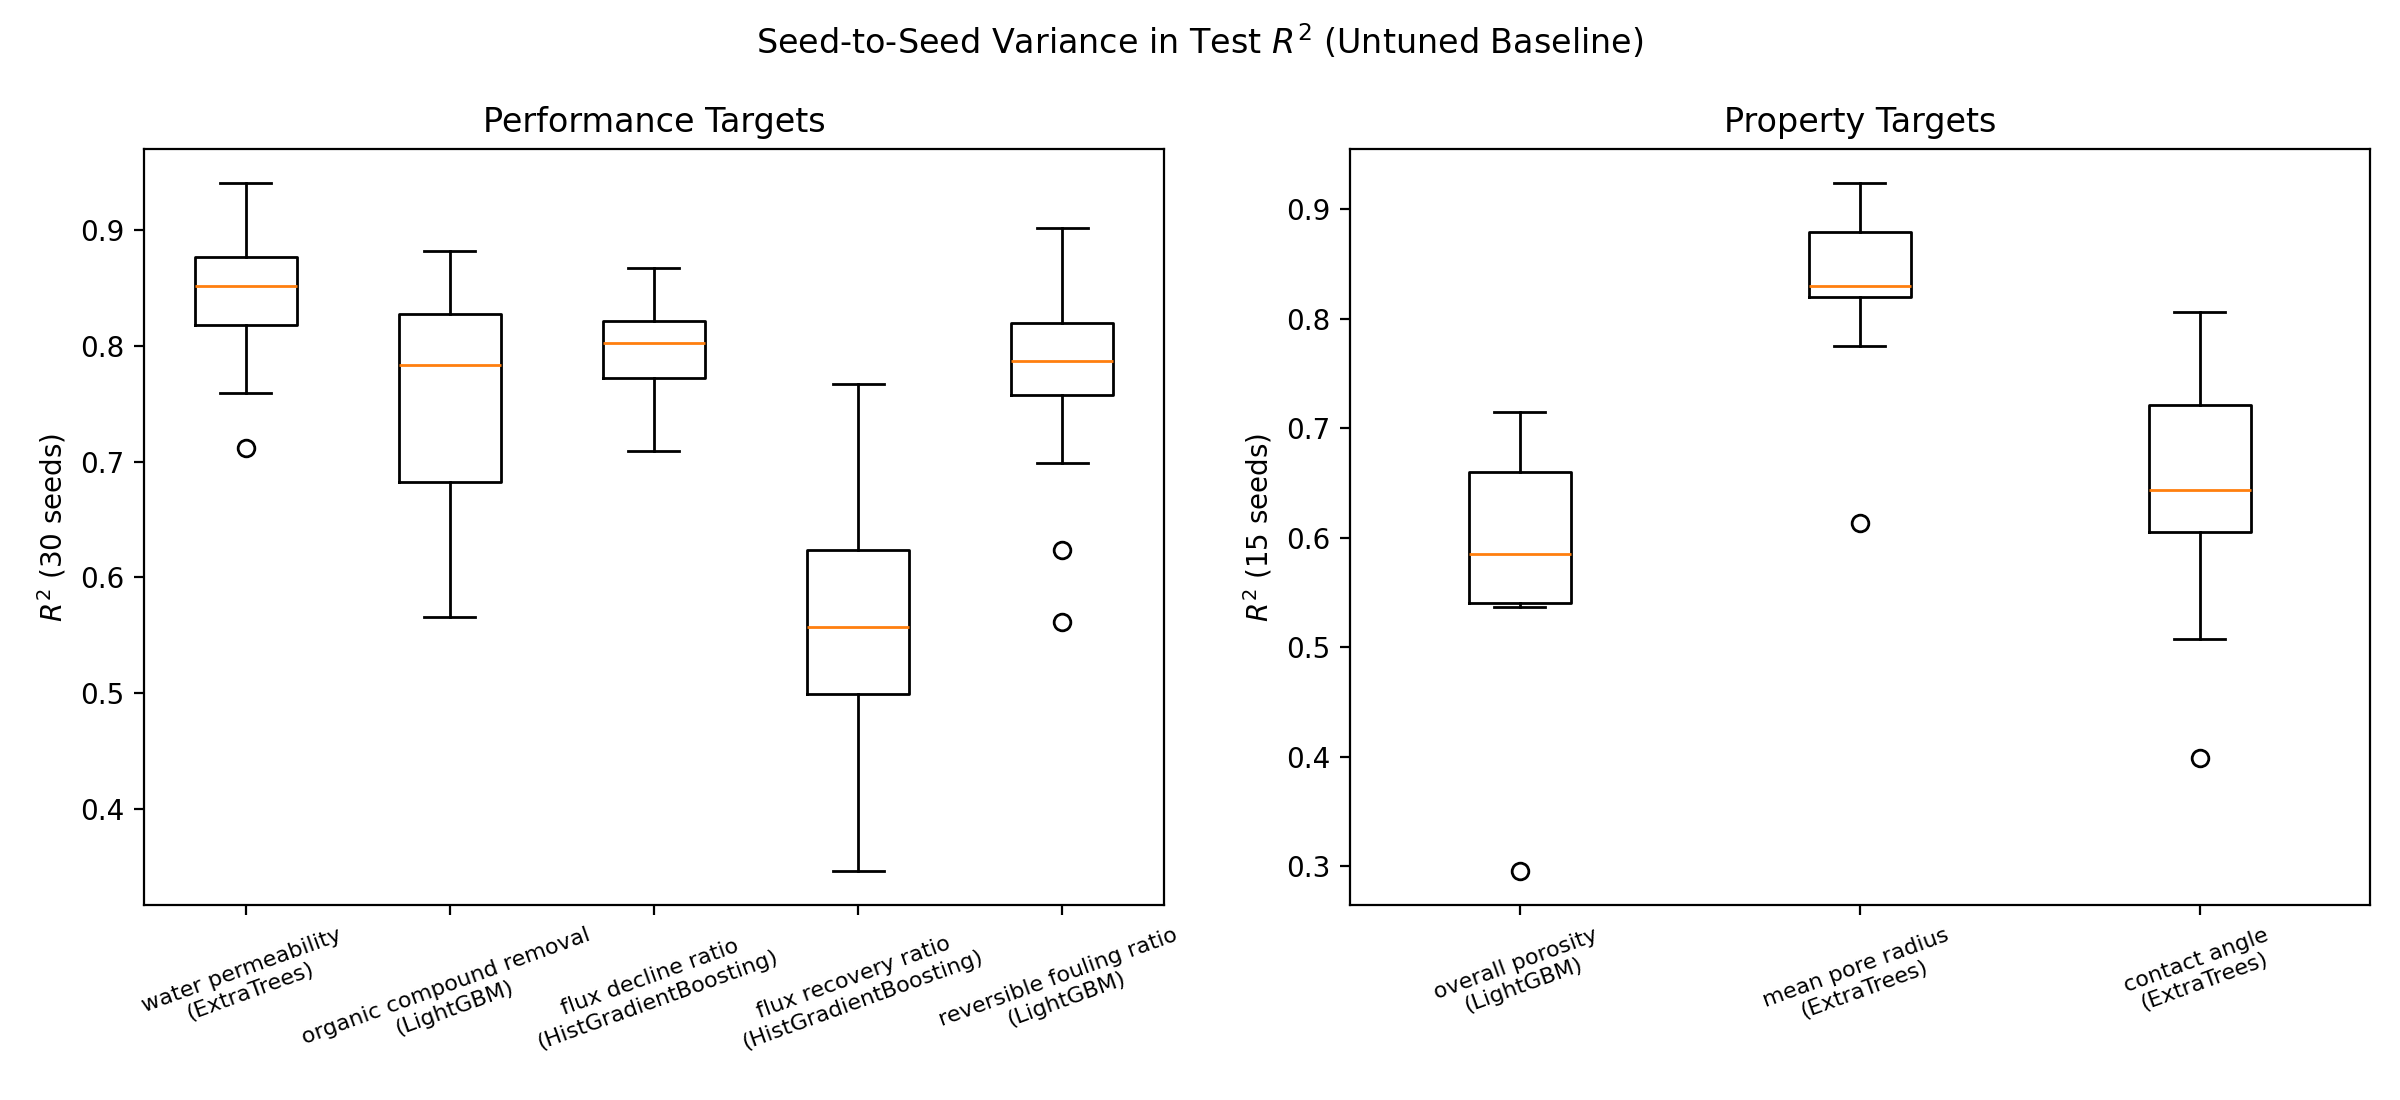
\includegraphics[width=0.9\textwidth]{figures/fig_seed_variance.png}
\caption{Distribution of untuned test $R^2$ across repeated random splits (30 seeds for performance targets; 15 seeds for property targets) for a representative top-performing model per target.}
\label{fig:seedvar}
\end{figure}

It is also necessary to state the remaining methodological limitations of this computational follow-up relative to the source paper. First, in the source paper, the Shapley additive explanations (SHAP) method was utilized to quantify feature importance and provide physical insights into membrane fabrication. \textbf{SHAP feature-importance analysis has not yet been executed on the new ensemble and GradientBoosting-based models developed in this study.} Consequently, while predictive accuracy has improved, the mechanistic interpretability (e.g., identifying the exact threshold of additive loading for optimal flux) remains to be mapped for the new architectures. This is a primary avenue for future work.

Second, while Gao et al.\ fabricated and tested three physical UF membranes to experimentally validate their ML predictions, \textbf{no experimental (wet-lab) validation membranes were fabricated in this computational study.} The improvements reported here are strictly confined to in-silico predictive metrics on the existing literature dataset.

Third, the parity plots (predicted vs.\ actual, train and test) for all eight targets are now included (Figures~\ref{fig:parity-performance} and~\ref{fig:parity-properties}); however, they surfaced the flux recovery ratio discrepancy discussed in Section 3.2, which remains unresolved rather than a clean confirmation of prior results.

Finally, it is important to note the statistical variance inherent in single-split evaluations. On this dataset size ($\sim$300 rows), a single 80/20 test split yields an $R^2$ that can swing by $\pm 0.05$ to $\pm 0.15$ depending on the random seed, consistent with the seed-to-seed standard deviations reported in Table~\ref{tab:baseline}. The single-split metrics (seed $= 1000$) are reported in Tables~\ref{tab:performance} and~\ref{tab:properties} for direct, apples-to-apples comparison with Gao et al.; the repeated-seed and DOI-grouped cross-validation results in Section 3.1 and above represent the more robust, leakage-aware view of generalization performance.

\section{Conclusion}

This work revisited the ML prediction of UF membrane performance using the benchmark dataset established by Gao et al.\ (2023). By replacing the original XGBoost/CatBoost algorithms with a diverse tree-ensemble zoo and introducing domain-informed feature engineering---specifically a chemical-family taxonomy for nanomaterial additives and physically motivated interaction terms---the proposed solution achieves superior predictive accuracy. After extending the Optuna hyperparameter search from three to nine candidate algorithms, resolving the discrepancy flagged by the sixteen-model baseline screen, and generating parity plots for all eight targets, the proposed solution beats the published benchmark $R^2$ on seven of eight targets (water permeability, organic compound removal, flux decline ratio, flux recovery ratio, reversible fouling ratio, overall porosity, and contact angle), with mean pore radius the sole remaining target behind benchmark, though with a narrowed gap. These results confirm that targeted feature engineering, per-target ensembling, and a genuinely exhaustive tuning search are highly effective levers for improving ML models in materials science -- while the flux recovery ratio discrepancy surfaced by the parity-plot sweep (Section 3.2) is a reminder that each round of re-tuning needs to be reconciled against, not simply substituted for, prior verified results.

At the same time, this update leaves a clear, concrete set of open items rather than a closed case: (1) the flux recovery ratio discrepancy between the previously verified HistGradientBoosting result ($R^2=0.638$) and the newer parity-plot sweep's LightGBM result ($R^2=0.619$) needs to be reconciled under an identical, fixed protocol before either number is treated as final; (2) train-set $R^2$/RMSE and test RMSE for most targets have not yet been captured alongside the parity plots and should be added in the next pass so the overfitting-gap analysis can be extended to them; (3) the DOI-grouped cross-validation results still describe only the original untuned sixteen-model screen and have not been re-run against any of the newer GradientBoosting-based or ensemble models, so whether the resolved and flagged discrepancies also shift under leakage-safe evaluation is unknown; and (4) AdaBoost, SVR (polynomial kernel), Lasso, PLS, KNN, BayesianRidge, and GaussianProcess remain untuned, since no hyperparameter search space has been defined for them, leaving open whether any of them would also outperform the currently reported best models if given the same tuning budget. Future work will additionally focus on executing SHAP analysis for mechanistic interpretability, implementing a two-stage predictive pipeline, and conducting wet-lab validation to confirm the in-silico predictions.

\section*{Associated Content}

\subsection*{Data Availability}

The Python scripts utilized for data loading, feature engineering, and leakage-safe Optuna tuning (\texttt{full\_pipeline\_part1\_data.py}, \texttt{full\_pipeline\_part2\_tuning.py}), the driver script used to reproduce the tuned and ensemble results across the full nine-model candidate set (\texttt{run\_full\_pipeline.py}), the raw JSON outputs containing the hyperparameter logs and tuned train/test metrics (\texttt{06\_train\_test\_batch1.json}, \texttt{08\_ensemble\_train\_metrics.json}), and the full sixteen-model untuned baseline screening results (\texttt{02\_baseline\_repeated\_ALL.csv}, \texttt{02\_baseline\_grouped\_ALL.csv}, \texttt{02\_baseline\_summary\_by\_model.csv}, \texttt{09\_baseline\_repeated\_properties\_ALL.csv}, \texttt{09\_baseline\_summary\_properties.csv}) are archived and available in the project repository. The underlying dataset is the same as that provided by Gao et al.\ (2023).

\textit{[INSERT LINK/DOI TO REPOSITORY HERE]}

\section*{Author Information}

\subsection*{Corresponding Author}
\textit{[Placeholder Name]} -- [Department], [University Name], [City], [State] [Zip Code], [Country]; Email: \texttt{email@address.com}

\subsection*{Authors}
Chirag Mishra -- [Department], [University Name], [City], [State] [Zip Code], [Country] \\
Pragya Kundu -- [Department], [University Name], [City], [State] [Zip Code], [Country] \\
Adi Shree Prod Rajesh Mahadeva -- [Department], [University Name], [City], [State] [Zip Code], [Country]

\subsection*{Author Contributions}
The manuscript was written through contributions of all authors. All authors have given approval to the final version of the manuscript.

\subsection*{Notes}
The authors declare no competing financial interest.

\section*{Acknowledgments}

\textit{[Placeholder for funding agencies, grants, or institutional support if applicable. E.g., This work was supported by the [Name of Funding Agency] under Grant [Number].]}

\begin{thebibliography}{9}

\bibitem{gao2023}
Gao, H.; Zhong, S.; Dangayach, R.; Chen, Y.
Understanding and Designing a High-Performance Ultrafiltration Membrane Using Machine Learning.
\textit{Environ. Sci. Technol.} \textbf{2023}, \textit{57} (46), 17831--17840.
DOI: \href{https://doi.org/10.1021/acs.est.2c05404}{10.1021/acs.est.2c05404}.

\end{thebibliography}

\end{document}
